% ============================================================
% HSBI Beamer — ISLP Lecture Series — IMPROVED EDITION
% Chapter 10: Deep Learning
% ============================================================
\documentclass[aspectratio=169,11pt]{beamer}
\usepackage[utf8]{inputenc}\usepackage[T1]{fontenc}\usepackage[english]{babel}
\usepackage{graphicx}\usepackage{booktabs}\usepackage{amsmath,amssymb,amsfonts}
\usepackage{mathtools}\usepackage{hyperref}\usepackage{xcolor}
\usepackage{verbatim}\usepackage{alltt}
\usepackage{tikz}\usetikzlibrary{calc,arrows.meta,positioning,shapes}
\usepackage{tcolorbox}\tcbuselibrary{skins}

\usetheme{Madrid}\usecolortheme{default}
\setbeamertemplate{navigation symbols}{}
\setbeamertemplate{footline}[frame number]
\setbeamertemplate{blocks}[rounded][shadow=false]
\setbeamertemplate{headline}{%
  \leavevmode\hbox{%
    \begin{beamercolorbox}[wd=\paperwidth,ht=2.2ex,dp=0.9ex]{section in head/foot}%
      {\fontsize{4.6}{5.2}\selectfont%
       \insertsectionnavigationhorizontal{\paperwidth}{}{\hskip0pt plus1filll}}%
    \end{beamercolorbox}}%
}
\setbeamerfont{section in head/foot}{size=\tiny}
\setbeamerfont{palette primary}{size=\tiny}
\setbeamerfont{palette tertiary}{size=\tiny}
\setbeamerfont{section in toc}{size=\footnotesize}

\usepackage{listings}
\definecolor{pyKw}{RGB}{0,0,180}\definecolor{pyStr}{RGB}{20,120,40}
\definecolor{pyCom}{RGB}{120,120,120}\definecolor{accent}{RGB}{38,70,140}
\lstdefinestyle{Pystyle}{language=Python,basicstyle=\ttfamily\footnotesize,
  keywordstyle=\color{pyKw}\bfseries,commentstyle=\color{pyCom}\itshape,
  stringstyle=\color{pyStr},showstringspaces=false,upquote=true,
  columns=fullflexible,breaklines=true,literate={~}{{$\sim$}}1}
\lstset{style=Pystyle}

\AtBeginSection[]{\begin{frame}{Outline}\footnotesize
  \tableofcontents[currentsection,sectionstyle=show/shaded,subsectionstyle=show/show/hide]
\end{frame}}

\newcommand{\islpsource}[1]{%
  \vfill\hfill{\tiny\itshape\color{gray}Source: #1 \textemdash{} ISLP, James et al.\ (2023).}\par
}

\newtcolorbox{takeaway}[1][Takeaway]{enhanced,colback=green!4,colframe=green!50!black,
  boxrule=0pt,leftrule=2.5pt,arc=2pt,fonttitle=\bfseries,title=#1,
  left=2mm,right=2mm,top=1mm,bottom=1mm}
\newtcolorbox{numexample}[1][Worked example]{enhanced,colback=orange!4,colframe=orange!70!black,
  boxrule=0pt,leftrule=2.5pt,arc=2pt,fonttitle=\bfseries,title=#1,
  left=2mm,right=2mm,top=1mm,bottom=1mm}
\newtcolorbox{readme}[1][How to read this]{enhanced,colback=blue!4,colframe=accent,
  boxrule=0pt,leftrule=2.5pt,arc=2pt,fonttitle=\bfseries,title=#1,
  left=2mm,right=2mm,top=1mm,bottom=1mm}

\title{Quantitative Research Methods}
\subtitle{Chapter 10: Deep Learning}
\author{Prof.\ Dr.\ Christoph Weisser}\institute{HSBI}
\date{Summer Semester 2026}\graphicspath{{images/}}

\newtcolorbox{exercise}[1][Exercise]{enhanced, fontupper=\footnotesize, colback=purple!4, colframe=purple!55!black, boxrule=0pt, leftrule=2.5pt, arc=2pt, fonttitle=\bfseries, title=#1, left=2mm, right=2mm, top=1mm, bottom=1mm}
\newtcolorbox{solutionbox}[1][Solution]{enhanced, fontupper=\footnotesize, colback=teal!5, colframe=teal!55!black, boxrule=0pt, leftrule=2.5pt, arc=2pt, fonttitle=\bfseries, title=#1, left=2mm, right=2mm, top=1mm, bottom=1mm}
\newtcolorbox{longexercise}[1][Extended exercise (15 min)]{enhanced, fontupper=\footnotesize, colback=violet!6, colframe=violet!55!black, boxrule=0pt, leftrule=3pt, arc=2pt, fonttitle=\bfseries, title=#1, left=2mm, right=2mm, top=1mm, bottom=1mm}

% Reclaim ~2pt of body height (custom nav headline makes full slides tip over by ~1.83pt)
\addtobeamertemplate{frametitle}{}{\vspace{-2pt}}

\newtcolorbox{labnote}[1][Run this live in the lab notebook]{enhanced, fontupper=\footnotesize, colback=cyan!7, colframe=cyan!45!black, boxrule=0pt, leftrule=3pt, arc=2pt, fonttitle=\bfseries, title=#1, left=2mm, right=2mm, top=1mm, bottom=1mm}

\begin{document}
\begin{frame}[plain]\titlepage\end{frame}

\begin{frame}{The course at a glance}
  \footnotesize
  \begin{center}
  \begin{tabular}{@{}c r l@{}}
    & \textbf{Lecture} & \textbf{Topic}\\
    \midrule
     & 1 & Ch.\ 1 + 2 --- Introduction; what is statistical learning \\
     & 2 & Ch.\ 2 --- Accuracy, bias--variance, Bayes classifier, KNN \\
     & 3--4 & Ch.\ 3 --- Linear regression (estimation, inference, diagnostics) \\
     & 5--6 & Ch.\ 4 --- Classification (logistic, LDA/QDA, naive Bayes, ROC) \\
     & 7 & Ch.\ 5 --- Resampling (validation, CV, bootstrap) \\
     & 8 & Ch.\ 6 --- Model selection and regularisation (ridge, lasso) \\
     & 9 & Ch.\ 7 --- Moving beyond linearity (splines, GAMs) \\
     & 10 & Ch.\ 8 --- Tree-based methods (trees, forests, boosting) \\
    $\blacktriangleright$ & \textbf{11} & \textbf{Ch.\ 10 --- Deep learning (MLPs, CNNs, training)} \\
     & 12 & Ch.\ 13 --- Multiple testing (FWER, FDR) \\
  \end{tabular}
  \end{center}
  \vspace{2pt}
  {\scriptsize Twelve sessions of 180 minutes. $\blacktriangleright$ marks today's chapter. Short exercises every $\sim$20 min; extended exercises every $\sim$45 min; each chapter has a companion lab notebook.}
\end{frame}


\begin{frame}{Contents}\footnotesize\tableofcontents[hideallsubsections]
  \vfill
  {\tiny Optional and advanced material is collected in the \textbf{appendix} at the end of the deck.}
\end{frame}

\begin{frame}{Notation in this chapter}
  \footnotesize
  \begin{center}
  \begin{tabular}{@{}ll@{}}
    \toprule
    \textbf{Symbol} & \textbf{Meaning} \\
    \midrule
    $X_j$, $p$ & input feature $j$; number of input features \\
    $K$ & number of hidden units in a layer \\
    $g(\cdot)$ & activation function (sigmoid, tanh, ReLU) \\
    $A_k$ & activation of hidden unit $k$: $A_k=g\big(w_{k0}+\sum_j w_{kj}X_j\big)$ \\
    $w_{kj}$, $w_{k0}$ & weight from input $j$ into hidden unit $k$; its bias \\
    $\beta_k$, $\beta_0$ & output weight of hidden unit $k$; output bias \\
    softmax & output activation $e^{z_m}/\sum_{m'} e^{z_{m'}}$ for multiclass labels \\
    $W$, $F$, $P$, $S$ & conv arithmetic: input width, filter size, padding, stride \\
    $\theta$ & all weights and biases of the network collectively \\
    $\eta$ & learning rate of (stochastic) gradient descent \\
    $\ell$ & per-observation loss (squared error, cross-entropy) \\
    \bottomrule
  \end{tabular}
  \end{center}
\end{frame}

\begin{frame}{Sources and references}
  \begin{block}{Primary textbook}
    James et al.\ (2023). \emph{An Introduction to Statistical Learning,
    with Applications in Python.} Springer.
  \end{block}
\end{frame}

\begin{frame}{Learning objectives}
  By the end of this chapter you will be able to:
  \begin{itemize}
    \item \textbf{Define} a single-layer and multilayer perceptron.
    \item \textbf{Explain} how convolutional networks exploit local
          structure and translation invariance.
    \item \textbf{Outline} recurrent networks and the basic
          transformer idea.
    \item \textbf{Train} a small network with stochastic gradient
          descent + backpropagation.
    \item \textbf{Reason} about when deep learning is worth it.
  \end{itemize}
\end{frame}


\begin{frame}{Roadmap of this chapter}
  \begin{takeaway}[A tour of modern deep learning]
    \begin{enumerate}
      \item Single-layer networks (logistic regression in disguise).
      \item Multilayer perceptrons.
      \item Convolutional networks for images.
      \item Recurrent networks and transformers for sequences.
      \item How they are trained (SGD, backprop) and regularised.
    \end{enumerate}
  \end{takeaway}
\end{frame}

% ============================================================
\section{Why now?}
% ============================================================

\begin{frame}{What is deep learning?}
  A renaissance of neural networks driven by GPUs, large labelled
  datasets, and algorithmic improvements (dropout, batch norm,
  attention).
  \begin{takeaway}
    Dominant in image, speech, and natural-language tasks. Less
    consistently dominant on small to medium tabular data --- where
    gradient-boosted trees often win.
  \end{takeaway}
\end{frame}


% ============================================================
\section{Single Layer}
% ============================================================

\begin{frame}{Single hidden layer}
  \[
    \boxed{\;
      \hat f(X) = \beta_0 + \sum_{k=1}^K \beta_k\,
                  g\!\left(w_{k0} + \sum_{j=1}^p w_{kj} X_j \right).
    \;}
  \]
  \begin{readme}[Reading the formula symbol by symbol]
    \begin{itemize}
      \item $X_j$: input feature $j$ ($j=1,\dots,p$); \ $g$: nonlinear activation
            (sigmoid, tanh, ReLU).
      \item $w_{kj}$: weight from input $j$ into hidden unit $k$; \ $w_{k0}$: its bias.
      \item $K$: number of hidden units (activations $A_k=g(\cdot)$); \ $\beta_k$:
            unit $k$'s output weight, $\beta_0$ the output bias.
    \end{itemize}
  \end{readme}
  \begin{takeaway}
    Read it inside-out: linear combination $\to$ nonlinearity $g$ $\to$ linear
    combination. Logistic regression $=$ this with $K=1$ and a sigmoid output.
  \end{takeaway}
\end{frame}

\begin{frame}{Single-layer network as a graph}
  \begin{center}
    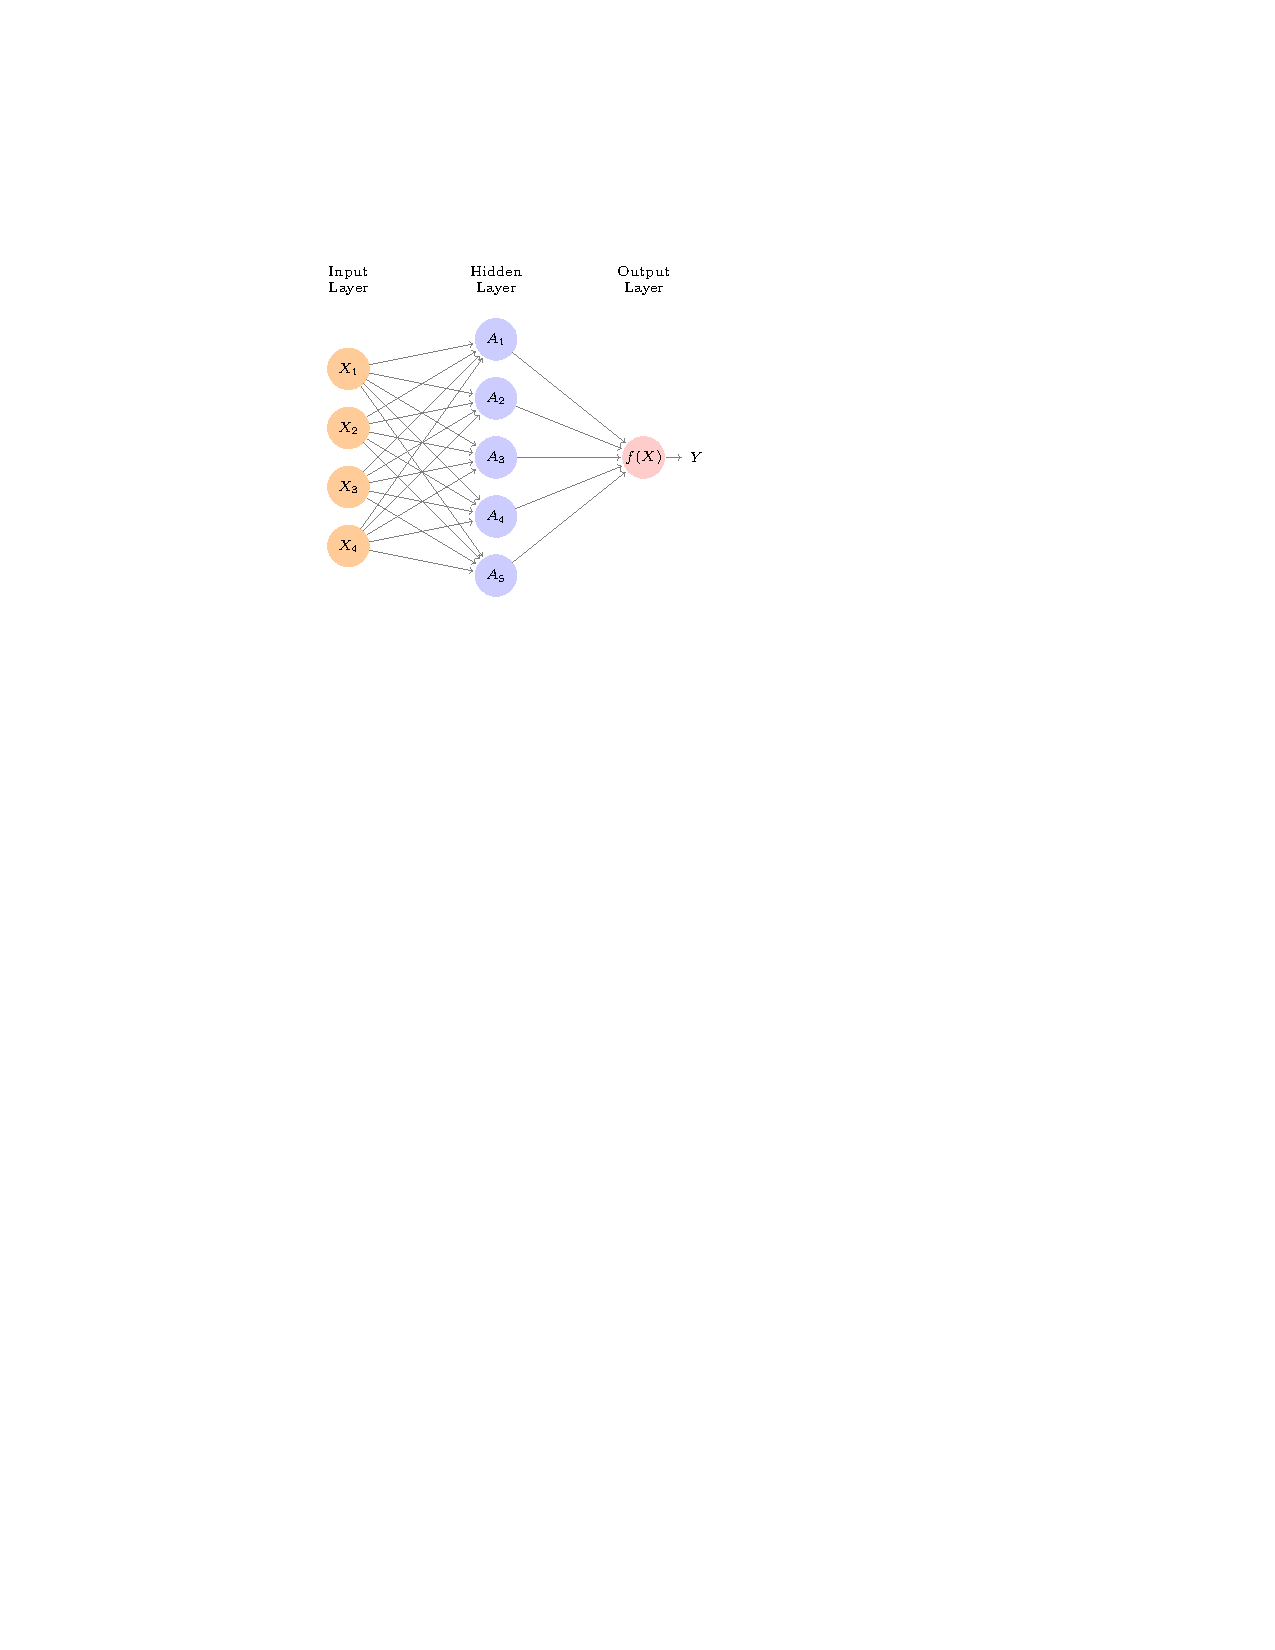
\includegraphics[width=0.62\textwidth,height=0.62\textheight,keepaspectratio]{10_1.pdf}
  \end{center}
  \islpsource{Figure 10.1}
\end{frame}

\begin{frame}{Feed-forward network as a labelled graph}
  \begin{center}
  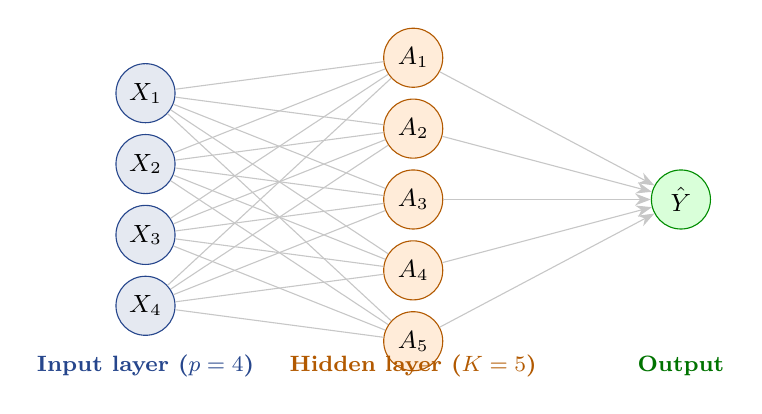
\begin{tikzpicture}[
      x=1.7cm,y=0.9cm,>={Stealth[length=2mm]},
      inp/.style={circle,draw=accent,fill=accent!12,minimum size=7.5mm,inner sep=0pt,font=\small},
      hid/.style={circle,draw=orange!70!black,fill=orange!15,minimum size=7.5mm,inner sep=0pt,font=\small},
      onode/.style={circle,draw=green!55!black,fill=green!15,minimum size=7.5mm,inner sep=0pt,font=\small},
      edge/.style={draw=black!22,line width=0.4pt}]
    \foreach \i in {1,...,4} \node[inp] (I\i) at (0,{2.5-(\i-1)}) {$X_{\i}$};
    \foreach \j in {1,...,5} \node[hid] (H\j) at (2,{3-(\j-1)}) {$A_{\j}$};
    \node[onode] (O) at (4,1) {$\hat Y$};
    \foreach \i in {1,...,4}\foreach \j in {1,...,5} \draw[edge] (I\i) -- (H\j);
    \foreach \j in {1,...,5} \draw[edge,->] (H\j) -- (O);
    \node[font=\footnotesize\bfseries,text=accent] at (0,-1.35) {Input layer ($p=4$)};
    \node[font=\footnotesize\bfseries,text=orange!70!black] at (2,-1.35) {Hidden layer ($K=5$)};
    \node[font=\footnotesize\bfseries,text=green!45!black] at (4,-1.35) {Output};
  \end{tikzpicture}
  \end{center}
  \begin{takeaway}
    Each hidden unit computes $A_k=g\!\left(w_{k0}+\sum_j w_{kj}X_j\right)$; the output linearly combines them, $\hat Y=\beta_0+\sum_k \beta_k A_k$. ``Fully connected'' means every input feeds every hidden unit.
  \end{takeaway}
\end{frame}

\begin{frame}{Anatomy of a single neuron}
  \begin{center}
  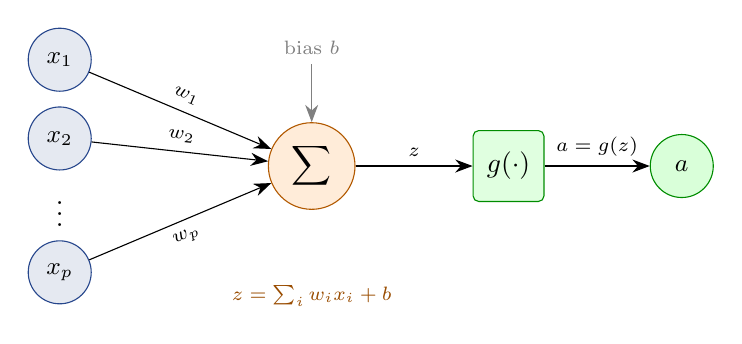
\begin{tikzpicture}[x=1cm,y=1cm,>={Stealth[length=2.2mm]},
      inp/.style={circle,draw=accent,fill=accent!12,minimum size=8mm,inner sep=1pt,font=\small},
      op/.style={circle,draw=orange!70!black,fill=orange!15,minimum size=11mm,inner sep=1pt},
      act/.style={rounded corners=2pt,draw=green!55!black,fill=green!12,minimum size=9mm,inner sep=4pt},
      onode/.style={circle,draw=green!55!black,fill=green!15,minimum size=8mm,inner sep=1pt,font=\small}]
    \node[inp] (x1) at (0,2)    {$x_1$};
    \node[inp] (x2) at (0,1)    {$x_2$};
    \node       (xd) at (0,0.15) {$\vdots$};
    \node[inp] (xp) at (0,-0.7) {$x_p$};
    \node[op]  (sum) at (3.2,0.65) {$\displaystyle\sum$};
    \node[act] (g)   at (5.7,0.65) {$g(\cdot)$};
    \node[onode] (a)   at (7.9,0.65) {$a$};
    \draw[->] (x1) -- node[above,sloped,font=\scriptsize]{$w_1$} (sum);
    \draw[->] (x2) -- node[above,sloped,font=\scriptsize]{$w_2$} (sum);
    \draw[->] (xp) -- node[below,sloped,font=\scriptsize]{$w_p$} (sum);
    \node[font=\scriptsize,text=gray] (b) at (3.2,2.15) {bias $b$};
    \draw[->,gray] (b) -- (sum);
    \draw[->] (sum) -- node[above,font=\scriptsize]{$z$} (g);
    \draw[->] (g) -- node[above,font=\scriptsize]{$a=g(z)$} (a);
    \node[font=\scriptsize,text=orange!60!black] at (3.2,-1.0) {$z=\sum_i w_i x_i+b$};
  \end{tikzpicture}
  \end{center}
  \begin{takeaway}
    A neuron takes a weighted sum of its inputs plus a bias, then applies a nonlinearity $g$. Composing layers of these units builds the network above.
  \end{takeaway}
\end{frame}

\begin{frame}{Activation functions: sigmoid vs.\ ReLU}
  \begin{readme}
    \begin{itemize}
      \item \textbf{Sigmoid}: $g(z) = 1/(1 + e^{-z})$, output in $(0,1)$. Saturates at
            $\pm\infty$ --- vanishing gradients.
      \item \textbf{Tanh}: $g(z)=\tanh(z)=\dfrac{e^{z}-e^{-z}}{e^{z}+e^{-z}}$, output in
            $(-1,1)$; same S-shape but zero-centred.
      \item \textbf{ReLU}: $g(z) = \max(0, z)$. Today's default ---
            sparser activations, faster training, better gradient flow.
    \end{itemize}
  \end{readme}
  \begin{takeaway}[Why it matters]
    The activation is the \emph{only} nonlinearity in the network: remove it and
    stacked layers collapse to one linear map (Exercise 10.2). ReLU is preferred
    because its gradient stays healthy through deep stacks.
  \end{takeaway}
\end{frame}

\begin{frame}{Activation functions and their gradients}
  \begin{center}
    
\includegraphics[width=0.92\textwidth,height=0.58\textheight,keepaspectratio]{ch10_activations.png}
  \end{center}
  \begin{takeaway}
    ReLU's gradient is $1$ on the active region, so signals pass undiminished; the sigmoid derivative never exceeds $0.25$ and vanishes in the tails --- the root of vanishing gradients in deep nets.
  \end{takeaway}
\end{frame}


% ------------------------------------------------------------
\begin{frame}{Exercise 10.1 --- Forward pass by hand [Math]}
\begin{exercise}
  Consider a single hidden-layer network with input
  $X = (X_1, X_2) = (2, 3)$, $K = 2$ ReLU hidden units, and a linear
  output. The parameters are
  \[
    \begin{aligned}
      &\text{Unit 1: } w_{1} = (1, 1),\; w_{10} = -4, \\
      &\text{Unit 2: } w_{2} = (-1, 2),\; w_{20} = 0,
    \end{aligned}
    \qquad
    \beta_0 = 1,\; \beta_1 = 2,\; \beta_2 = -1 .
  \]
  \begin{enumerate}
    \item Compute the two hidden activations $A_1, A_2$ using
          $g(z) = \max(0, z)$.
    \item Compute the network output $\hat f(X)$.
    \item Treating the output as a binary-classification logit, apply
          the sigmoid $\sigma(z) = 1/(1 + e^{-z})$ to obtain
          $\Pr(Y = 1 \mid X)$ and give the predicted class at
          threshold $0.5$.
  \end{enumerate}
\end{exercise}
\end{frame}

\begin{frame}{Solution --- Exercise 10.1 (1/2)}
\begin{solutionbox}
  \textbf{Method.} Work inside-out: each hidden unit first forms its affine
  pre-activation $z_k = w_{k0} + w_k^\top X$, then applies the nonlinearity
  $g(z) = \max(0, z)$ element-wise.

  \medskip
  \textbf{Step 1 --- pre-activations.}
  \[
    z_1 = w_{10} + w_1^\top X = -4 + (1)(2) + (1)(3) = -4 + 5 = 1,
  \]
  \[
    z_2 = w_{20} + w_2^\top X = 0 + (-1)(2) + (2)(3) = -2 + 6 = 4 .
  \]
  \textbf{Step 2 --- ReLU activations.} Both pre-activations are positive,
  so ReLU passes them through unchanged:
  \[
    A_1 = \max(0, 1) = 1, \qquad A_2 = \max(0, 4) = 4 .
  \]
  \textit{Common mistake: forgetting the bias $w_{10} = -4$ and reporting
  $z_1 = 5$ --- always add the bias before applying $g$.}
\end{solutionbox}
\end{frame}

\begin{frame}{Solution --- Exercise 10.1 (2/2)}
\begin{solutionbox}
  \textbf{Step 3 --- output.}
  \[
    \hat f(X) = \beta_0 + \beta_1 A_1 + \beta_2 A_2
             = 1 + (2)(1) + (-1)(4) = -1 .
  \]
  \textbf{Step 4 --- sigmoid probability.}
  \[
    \sigma(-1) = \frac{1}{1 + e^{1}} = \frac{1}{1 + 2.718} = 0.269 .
  \]
  Since $0.269 < 0.5$, the predicted class is $Y = 0$.
  \emph{Shortcut check:} $\sigma$ is monotone, so
  $\sigma(z) \ge 0.5 \iff z \ge 0$ --- the negative logit $-1$ already
  announces class $0$ before any arithmetic.

  \medskip
  \textbf{Take-away.} A forward pass is just alternating affine maps
  and element-wise nonlinearities. Note that if $z_1$ had been
  negative, ReLU would have set that unit to exactly $0$, ``switching
  it off''.

  \medskip
  \textit{Common mistake: squashing the hidden units with the sigmoid too ---
  here $g$ is ReLU; only the output logit is passed through $\sigma$.}
\end{solutionbox}
\end{frame}

\begin{frame}{Exercise 10.2 --- Why nonlinearity? [Concept]}
\begin{exercise}
  \begin{enumerate}
    \item Show algebraically that a two-layer network with
          \emph{identity} activations,
          $A^{(1)} = W^{(1)} X + b^{(1)}$ and
          $\hat Y = W^{(2)} A^{(1)} + b^{(2)}$, is equivalent to a
          single linear model. What does this imply for stacking
          layers without a nonlinearity?
    \item Give two concrete advantages of ReLU over the sigmoid
          activation.
    \item Explain the ``vanishing gradient'' problem of the sigmoid
          using its derivative.
  \end{enumerate}
\end{exercise}
\end{frame}

\begin{frame}{Solution --- Exercise 10.2 (1/2)}
\begin{solutionbox}
  \textbf{Part 1 --- linear collapse.} Substituting,
  \[
    \hat Y = W^{(2)}\big(W^{(1)} X + b^{(1)}\big) + b^{(2)}
           = \underbrace{\big(W^{(2)} W^{(1)}\big)}_{W'} X
             + \underbrace{\big(W^{(2)} b^{(1)} + b^{(2)}\big)}_{b'}
           = W' X + b' .
  \]
  This is a single affine (linear) map. Hence \emph{any} number of
  linear layers collapses to one linear layer: depth buys nothing
  without a nonlinearity. Nonlinear $g$ is what lets a network
  approximate curved decision boundaries and functions.
  \textit{Common mistake: hoping the biases add flexibility --- they
  collapse too, into the single vector $b'$.}

  \medskip
  \textbf{Part 2 --- ReLU advantages.}
  \begin{itemize}
    \item \emph{No saturation for $z > 0$}: the derivative is exactly
          $1$, so gradients pass through undiminished, enabling deep
          networks to train.
    \item \emph{Cheap and sparse}: $\max(0, z)$ is a single
          comparison; it also sets many units to exactly $0$, giving
          sparse, efficient representations.
  \end{itemize}
\end{solutionbox}
\end{frame}

\begin{frame}{Solution --- Exercise 10.2 (2/2)}
\begin{solutionbox}
  \textbf{Part 3 --- vanishing gradients.} For
  $\sigma(z) = 1/(1 + e^{-z})$ the derivative is
  \[
    \sigma'(z) = \sigma(z)\big(1 - \sigma(z)\big) \le 0.25 ,
  \]
  with its maximum at $z = 0$, where $\sigma'(0) = 0.5 \times 0.5 = 0.25$,
  and $\sigma'(z) \to 0$ as $|z| \to \infty$ (already at $z = 5$,
  $\sigma' \approx 0.0066$). In backpropagation the
  layer gradients \emph{multiply}, so through $L$ sigmoid layers the
  signal shrinks by up to $0.25^{L}$ --- for $L = 10$ that is
  $0.25^{10} \approx 10^{-6}$: it vanishes, and early
  layers barely learn. ReLU's derivative of $1$ on the active region
  avoids this.

  \medskip
  \textbf{Interpretation.} Vanishing gradients are a property of the
  \emph{product} of many small local derivatives, not of any one layer:
  each sigmoid layer is harmless alone, but ten in a row mute the error
  signal reaching the early weights.

  \medskip
  \textit{Common mistake: evaluating the derivative as
  $\sigma'(z) = z(1 - z)$ --- the formula plugs in the \emph{output}
  $\sigma(z)$, not the pre-activation $z$ itself.}
\end{solutionbox}
\end{frame}

% ------------------------------------------------------------
% EXTENDED (INTEGRATIVE) EXERCISE 10.1 --- forward pass + backprop
\begin{frame}{Extended Exercise 10.1 --- Tiny network by hand [Math]}
\begin{longexercise}
  A network has two inputs, one hidden layer of \textbf{two ReLU units}, and a single
  \textbf{sigmoid} output. Take input $x=(x_1,x_2)=(1,2)$ and target $y=0$, with
  \[
    \text{Unit 1: } w_1=(1,1),\ b_1=-1;\qquad
    \text{Unit 2: } w_2=(0,1),\ b_2=0;
  \]
  \[
    \text{logit } s=v_1a_1+v_2a_2+c,\quad v=(1,-\tfrac12),\ c=0,\quad
    \hat y=\sigma(s).
  \]
  Use squared-error loss $L=\tfrac12(\hat y-y)^2$ and learning rate $\eta=0.1$.
  \begin{enumerate}
    \item \textbf{Forward pass:} find $z_k$, $a_k=\max(0,z_k)$, the logit $s$,
          $\hat y=\sigma(s)$ and the loss $L$.
    \item \textbf{Backprop:} write the chain rule for $\partial L/\partial w_{11}$
          (the $x_1\!\to\!$unit-1 weight) and evaluate each factor.
    \item \textbf{Update:} take one gradient-descent step on $w_{11}$ and interpret it.
  \end{enumerate}
\end{longexercise}
\end{frame}

\begin{frame}{Solution --- Extended Exercise 10.1 (1/3)}
\begin{solutionbox}[Forward pass]
  \textbf{Method.} Alternate affine maps and nonlinearities,
  $z_k \to a_k \to s \to \hat y \to L$, and keep every intermediate value ---
  backpropagation will reuse each one.

  \medskip
  \textbf{Hidden pre-activations and ReLU.}
  \[
    z_1=(1)(1)+(1)(2)-1=2,\qquad a_1=\max(0,2)=2,
  \]
  \[
    z_2=(0)(1)+(1)(2)+0=2,\qquad a_2=\max(0,2)=2.
  \]
  \textbf{Output logit and sigmoid.}
  \[
    s=(1)(2)+(-\tfrac12)(2)+0=1,\qquad
    \hat y=\sigma(1)=\frac{1}{1+e^{-1}}=\frac{1}{1+0.368}=0.731 .
  \]
  \textbf{Squared-error loss} (target $y=0$, so the error is $\hat y$ itself):
  \[
    L=\tfrac12(\hat y-y)^2=\tfrac12(0.731)^2=0.267 .
  \]
\end{solutionbox}
\end{frame}

\begin{frame}{Solution --- Extended Exercise 10.1 (2/3)}
\begin{solutionbox}[Backpropagation: the chain rule]
  The weight $w_{11}$ reaches the loss along
  $z_1\!\to\!a_1\!\to\!s\!\to\!\hat y\!\to\!L$:
  \[
    \frac{\partial L}{\partial w_{11}}
    =\frac{\partial L}{\partial \hat y}\,
     \frac{\partial \hat y}{\partial s}\,
     \frac{\partial s}{\partial a_1}\,
     \frac{\partial a_1}{\partial z_1}\,
     \frac{\partial z_1}{\partial w_{11}} .
  \]
  Evaluate each factor:
  \[
    \frac{\partial L}{\partial \hat y}=\hat y-y=0.731,\qquad
    \frac{\partial \hat y}{\partial s}=\sigma(s)\big(1-\sigma(s)\big)=(0.731)(0.269)=0.197,
  \]
  \[
    \frac{\partial s}{\partial a_1}=v_1=1,\qquad
    \frac{\partial a_1}{\partial z_1}=\mathbf{1}\{z_1>0\}=1,\qquad
    \frac{\partial z_1}{\partial w_{11}}=x_1=1 .
  \]
  The first two factors combine into the reusable ``error signal''
  $\delta=(\hat y-y)\,\sigma'(s)=0.731\times0.197=0.144$.
  \textit{Common mistake: evaluating $\sigma'(s)$ by plugging $s=1$ into
  $u(1-u)$ --- the $u$ in $\sigma'(s)=u(1-u)$ is $u=\sigma(s)=0.731$.}
\end{solutionbox}
\end{frame}

\begin{frame}{Solution --- Extended Exercise 10.1 (3/3)}
\begin{solutionbox}[Gradient step and interpretation]
  \textbf{Multiply the factors.}
  \[
    \frac{\partial L}{\partial w_{11}}
      =0.731\times0.197\times1\times1\times1=0.144 .
  \]
  \textbf{Gradient-descent step} ($\eta=0.1$):
  \[
    w_{11}\leftarrow w_{11}-\eta\,\frac{\partial L}{\partial w_{11}}
      =1-0.1(0.144)=0.986 .
  \]
  \emph{Check:} redoing the forward pass with $w_{11}=0.986$ gives
  $s=0.986$, $\hat y=0.728$, $L=0.265<0.267$ --- the loss indeed fell.

  \smallskip
  \textbf{Interpretation.} $\hat y=0.731$ overshoots the target $0$, so the gradient is
  positive and the step \emph{lowers} $w_{11}$, pulling $\hat y$ down. The shared factor
  $\delta=(\hat y-y)\,\sigma'(s)=0.144$ is the output ``error signal'': backprop reuses it
  for \emph{every} weight, multiplying only by that weight's local input. Had $z_1$ been
  negative, $\partial a_1/\partial z_1=0$ would kill the gradient --- a ``dead'' ReLU unit
  stops learning.
\end{solutionbox}
\end{frame}

% ============================================================
\section{Multilayer}
% ============================================================

\begin{frame}{Multilayer perceptron (MLP)}
  Stack hidden layers:
  \begin{block}{Forward pass}
    \begin{align*}
      A^{(1)} &= g(W^{(1)} X + b^{(1)}), \\
      A^{(2)} &= g(W^{(2)} A^{(1)} + b^{(2)}), \\
              &\vdots \\
      \hat Y  &= h(W^{(L)} A^{(L-1)} + b^{(L)}).
    \end{align*}
  \end{block}
  \begin{readme}
    $h$ is the output activation: identity for regression, softmax
    for multiclass classification.
  \end{readme}
\end{frame}

\begin{frame}{MLP as a graph: stacking hidden layers}
  \begin{center}
    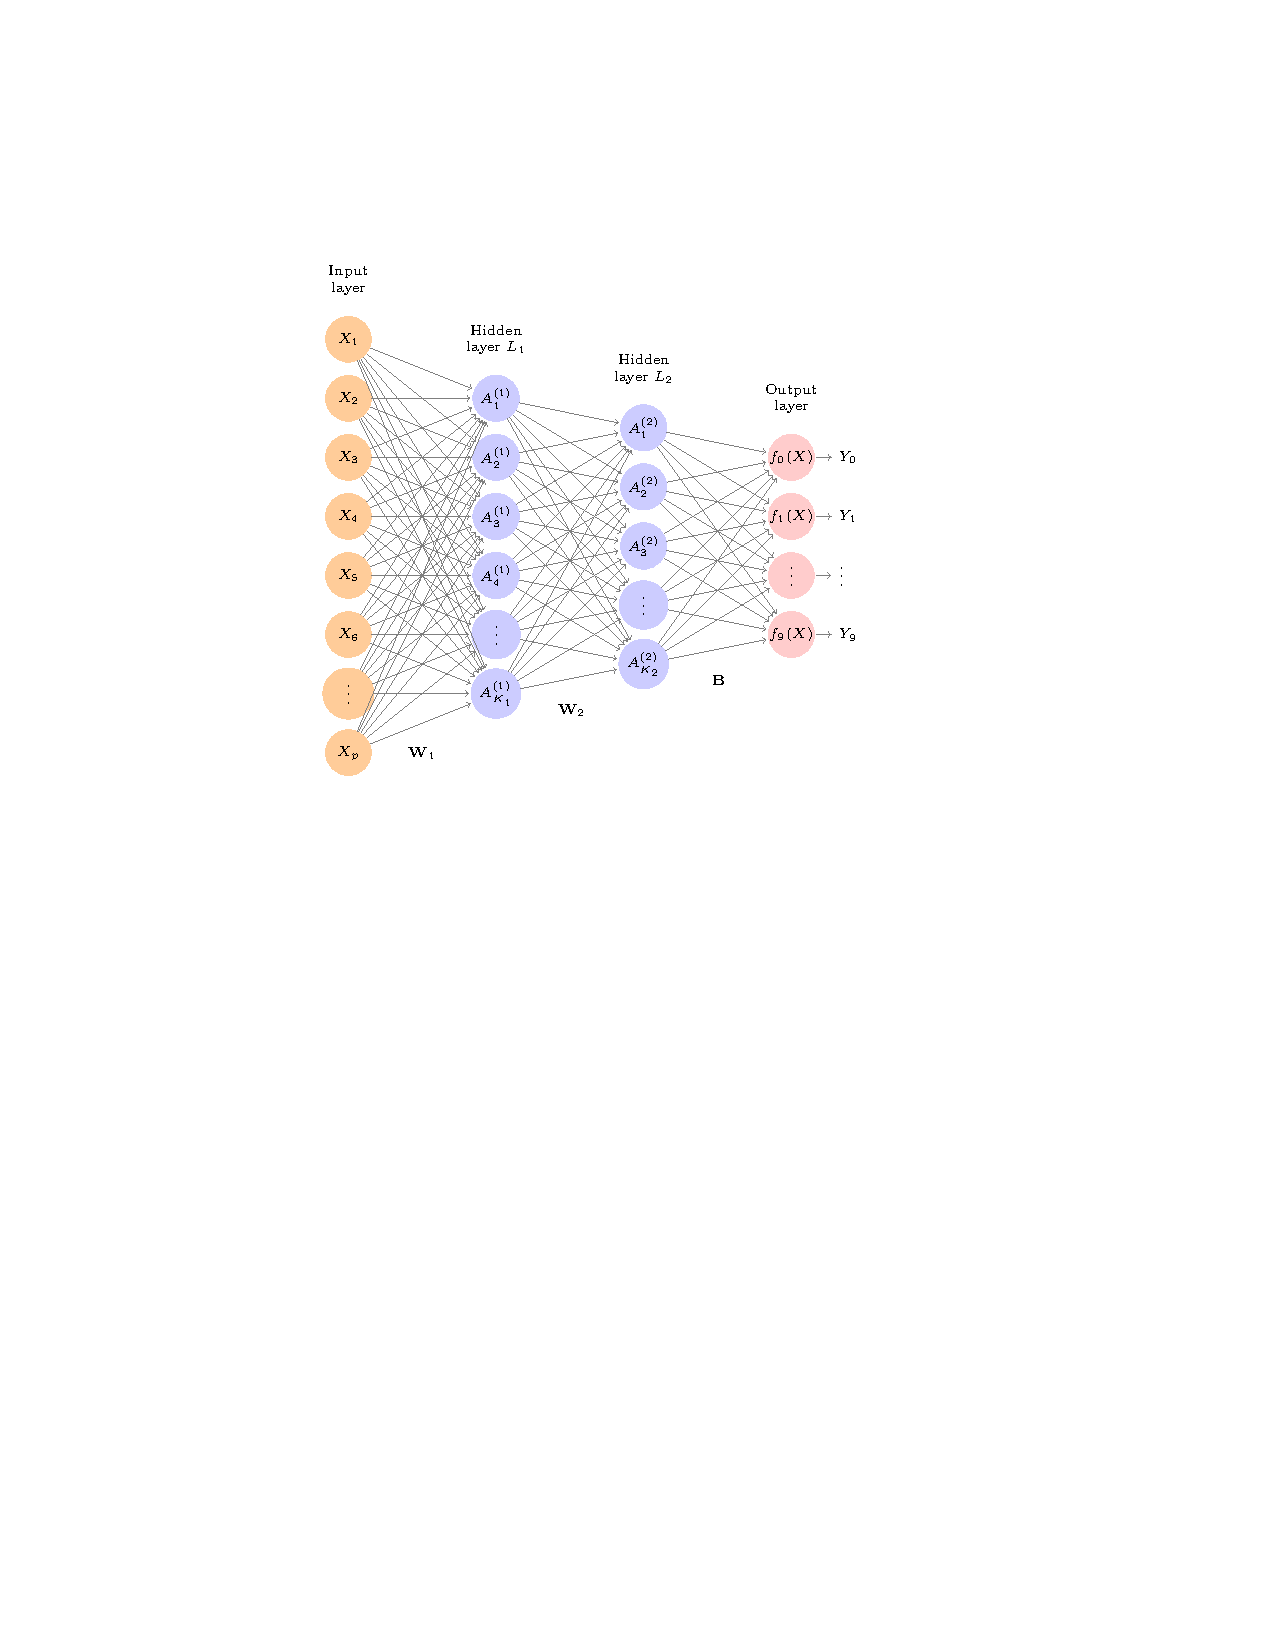
\includegraphics[width=0.85\textwidth,height=0.54\textheight,keepaspectratio]{10_4.pdf}
  \end{center}
  \begin{takeaway}
    Each layer transforms the previous layer's features; stacking them lets the
    network build progressively more abstract representations from the raw inputs.
  \end{takeaway}
  \islpsource{Figure 10.4}
\end{frame}


% ------------------------------------------------------------
\begin{frame}{Exercise 10.3 --- Counting parameters [Math]}
\begin{exercise}
  A fully-connected classifier has the architecture
  \[
    \underbrace{10}_{\text{inputs}}
    \;\rightarrow\; 32 \;\rightarrow\; 16
    \;\rightarrow\; \underbrace{3}_{\text{softmax outputs}},
  \]
  where every hidden and output unit has a bias term.
  \begin{enumerate}
    \item State the general rule for the number of trainable
          parameters in a dense layer with $n_{\text{in}}$ inputs and
          $n_{\text{out}}$ units.
    \item Count the parameters layer by layer.
    \item Give the total.
  \end{enumerate}
\end{exercise}
\end{frame}

\begin{frame}{Solution --- Exercise 10.3 (1/2)}
\begin{solutionbox}
  \textbf{Step 1 --- the rule and why.} A dense layer maps
  $n_{\text{in}} \to n_{\text{out}}$: every input--output pair carries one
  weight (an $n_{\text{in}} \times n_{\text{out}}$ matrix), and each output
  unit adds one bias, so
  \[
    \#\text{params} = n_{\text{in}}\, n_{\text{out}} + n_{\text{out}} .
  \]
  The input layer itself holds \emph{no} parameters --- it only passes the
  feature values forward.

  \medskip
  \textbf{Step 2 --- layer by layer.}
  \[
    \begin{aligned}
      \text{Layer 1 } (10 \to 32): &\quad 10 \times 32 + 32 = 320 + 32 = 352, \\
      \text{Layer 2 } (32 \to 16): &\quad 32 \times 16 + 16 = 512 + 16 = 528, \\
      \text{Output } (16 \to 3):   &\quad 16 \times 3  + 3  = 48  + 3  = 51 .
    \end{aligned}
  \]
\end{solutionbox}
\end{frame}

\begin{frame}{Solution --- Exercise 10.3 (2/2)}
\begin{solutionbox}
  \textbf{Step 3 --- total.}
  \[
    352 + 528 + 51 = \boxed{931} \text{ trainable parameters.}
  \]
  \textbf{Where the parameters live.} The three blocks contribute
  \[
    352/931 \approx 38\%, \qquad 528/931 \approx 57\%, \qquad 51/931 \approx 5\%:
  \]
  the $32 \to 16$ block dominates because its weight \emph{product}
  $n_{\text{in}} n_{\text{out}}$ is largest, while all biases together
  ($32 + 16 + 3 = 51$) are almost a rounding error.

  \medskip
  \textbf{Take-away.} Biases add only $n_{\text{out}}$ each but are
  easy to forget. Most parameters live in the widest weight matrices,
  which is why hidden-layer width drives model size --- and why parameter
  counting is a quick sanity check before training.

  \medskip
  \textit{Common mistake: attaching parameters to the $10$ input units, or
  dropping the $+n_{\text{out}}$ bias term --- both corrupt the total.}
\end{solutionbox}
\end{frame}

% ============================================================
\section{CNNs}
% ============================================================

\begin{frame}{Why convolutions?}
  Image data have local, translation-invariant structure.
  \begin{takeaway}
    A cat remains a cat shifted by 10 pixels. Fully-connected networks
    ignore this and need much more data.
  \end{takeaway}
  \begin{readme}[Two key layer types]
    \begin{itemize}
      \item \textbf{Convolutional layers}: each unit looks at a small
            patch of the input; weights are shared across positions.
      \item \textbf{Pooling layers}: down-sample (max or average) for
            translation tolerance.
    \end{itemize}
  \end{readme}
\end{frame}

\begin{frame}{The convolution operation}
  \begin{center}
  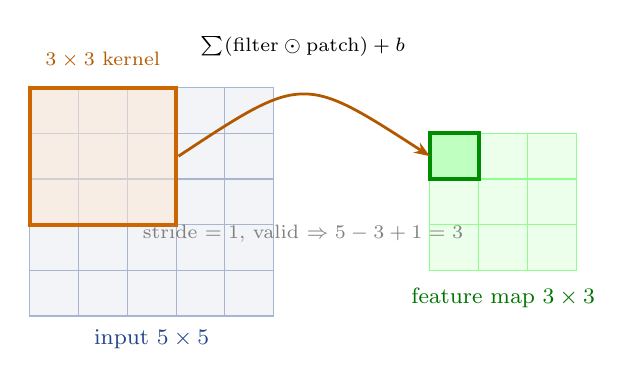
\begin{tikzpicture}[x=0.62cm,y=0.58cm,>={Stealth[length=2mm]},font=\small]
    \foreach \r in {0,...,4}\foreach \c in {0,...,4}
      \draw[fill=accent!6,draw=accent!40] (\c,-\r) rectangle ++(1,-1);
    \draw[draw=orange!80!black,line width=1.4pt,fill=orange!18,fill opacity=0.5]
      (0,0) rectangle (3,-3);
    \node[font=\scriptsize,text=orange!70!black] at (1.5,0.6) {$3\times3$ kernel};
    \node[font=\footnotesize,text=accent] at (2.5,-5.5) {input $5\times5$};
    \begin{scope}[shift={(8.2,-1)}]
      \foreach \r in {0,...,2}\foreach \c in {0,...,2}
        \draw[fill=green!8,draw=green!45] (\c,-\r) rectangle ++(1,-1);
      \draw[draw=green!55!black,line width=1.4pt,fill=green!25] (0,0) rectangle (1,-1);
      \node[font=\footnotesize,text=green!45!black] at (1.5,-3.6) {feature map $3\times3$};
    \end{scope}
    \draw[->,line width=1pt,orange!70!black] (3.05,-1.5) .. controls (5.6,0.3) .. (8.2,-1.5);
    \node[font=\scriptsize] at (5.6,0.9) {$\sum(\text{filter}\odot\text{patch})+b$};
    \node[font=\scriptsize,text=gray] at (5.6,-3.2) {stride $=1$, valid $\Rightarrow 5-3+1=3$};
  \end{tikzpicture}
  \end{center}
  \begin{takeaway}
    Each output cell is a dot product of the shared-weight filter with a local input patch. Weight sharing plus locality make convolutional neural networks (CNNs) data-efficient for images.
  \end{takeaway}
\end{frame}

\begin{frame}{Max-pooling: downsampling by local maxima}
  \begin{center}
  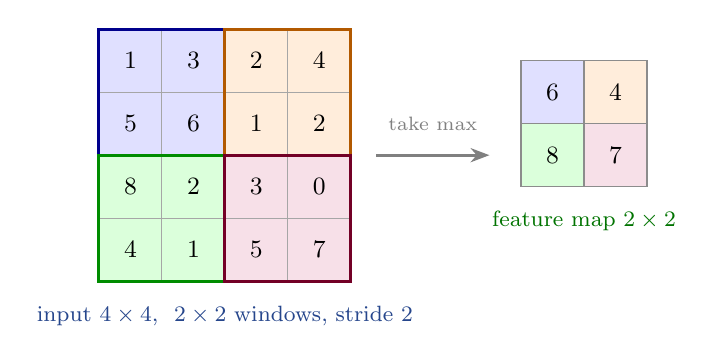
\begin{tikzpicture}[x=0.8cm,y=0.8cm,>={Stealth[length=2.4mm]},font=\small]
    \fill[blue!12]   (0,0) rectangle (2,-2);
    \fill[orange!14] (2,0) rectangle (4,-2);
    \fill[green!14]  (0,-2) rectangle (2,-4);
    \fill[purple!12] (2,-2) rectangle (4,-4);
    \foreach \r in {0,...,3}\foreach \c in {0,...,3} \draw[black!35] (\c,-\r) rectangle ++(1,-1);
    \foreach \c/\r/\v in {0/0/1,1/0/3,2/0/2,3/0/4, 0/1/5,1/1/6,2/1/1,3/1/2,
                          0/2/8,1/2/2,2/2/3,3/2/0, 0/3/4,1/3/1,2/3/5,3/3/7}
      \node at (\c+0.5,-\r-0.5) {\v};
    \draw[blue!55!black,line width=1.1pt]   (0,0) rectangle (2,-2);
    \draw[orange!70!black,line width=1.1pt] (2,0) rectangle (4,-2);
    \draw[green!55!black,line width=1.1pt]  (0,-2) rectangle (2,-4);
    \draw[purple!60!black,line width=1.1pt] (2,-2) rectangle (4,-4);
    \node[font=\footnotesize,text=accent] at (2,-4.55) {input $4\times4$, \ $2\times2$ windows, stride $2$};
    \draw[->,line width=1pt,gray] (4.4,-2) -- (6.2,-2);
    \node[font=\scriptsize,text=gray] at (5.3,-1.5) {take max};
    \begin{scope}[shift={(6.7,-0.5)}]
      \fill[blue!12]   (0,0) rectangle (1,-1);
      \fill[orange!14] (1,0) rectangle (2,-1);
      \fill[green!14]  (0,-1) rectangle (1,-2);
      \fill[purple!12] (1,-1) rectangle (2,-2);
      \foreach \c in {0,1}\foreach \r in {0,1}\draw[black!45] (\c,-\r) rectangle ++(1,-1);
      \node at (0.5,-0.5){6}; \node at (1.5,-0.5){4};
      \node at (0.5,-1.5){8}; \node at (1.5,-1.5){7};
      \node[font=\footnotesize,text=green!45!black] at (1,-2.55) {feature map $2\times2$};
    \end{scope}
  \end{tikzpicture}
  \end{center}
  \begin{takeaway}
    Each coloured window is replaced by its maximum, shrinking $H,W$ by the stride
    while keeping the depth. This buys small-shift tolerance and cuts computation ---
    and pooling has \emph{no} trainable parameters.
  \end{takeaway}
\end{frame}

\begin{frame}{A simple CNN architecture}
  \begin{center}
    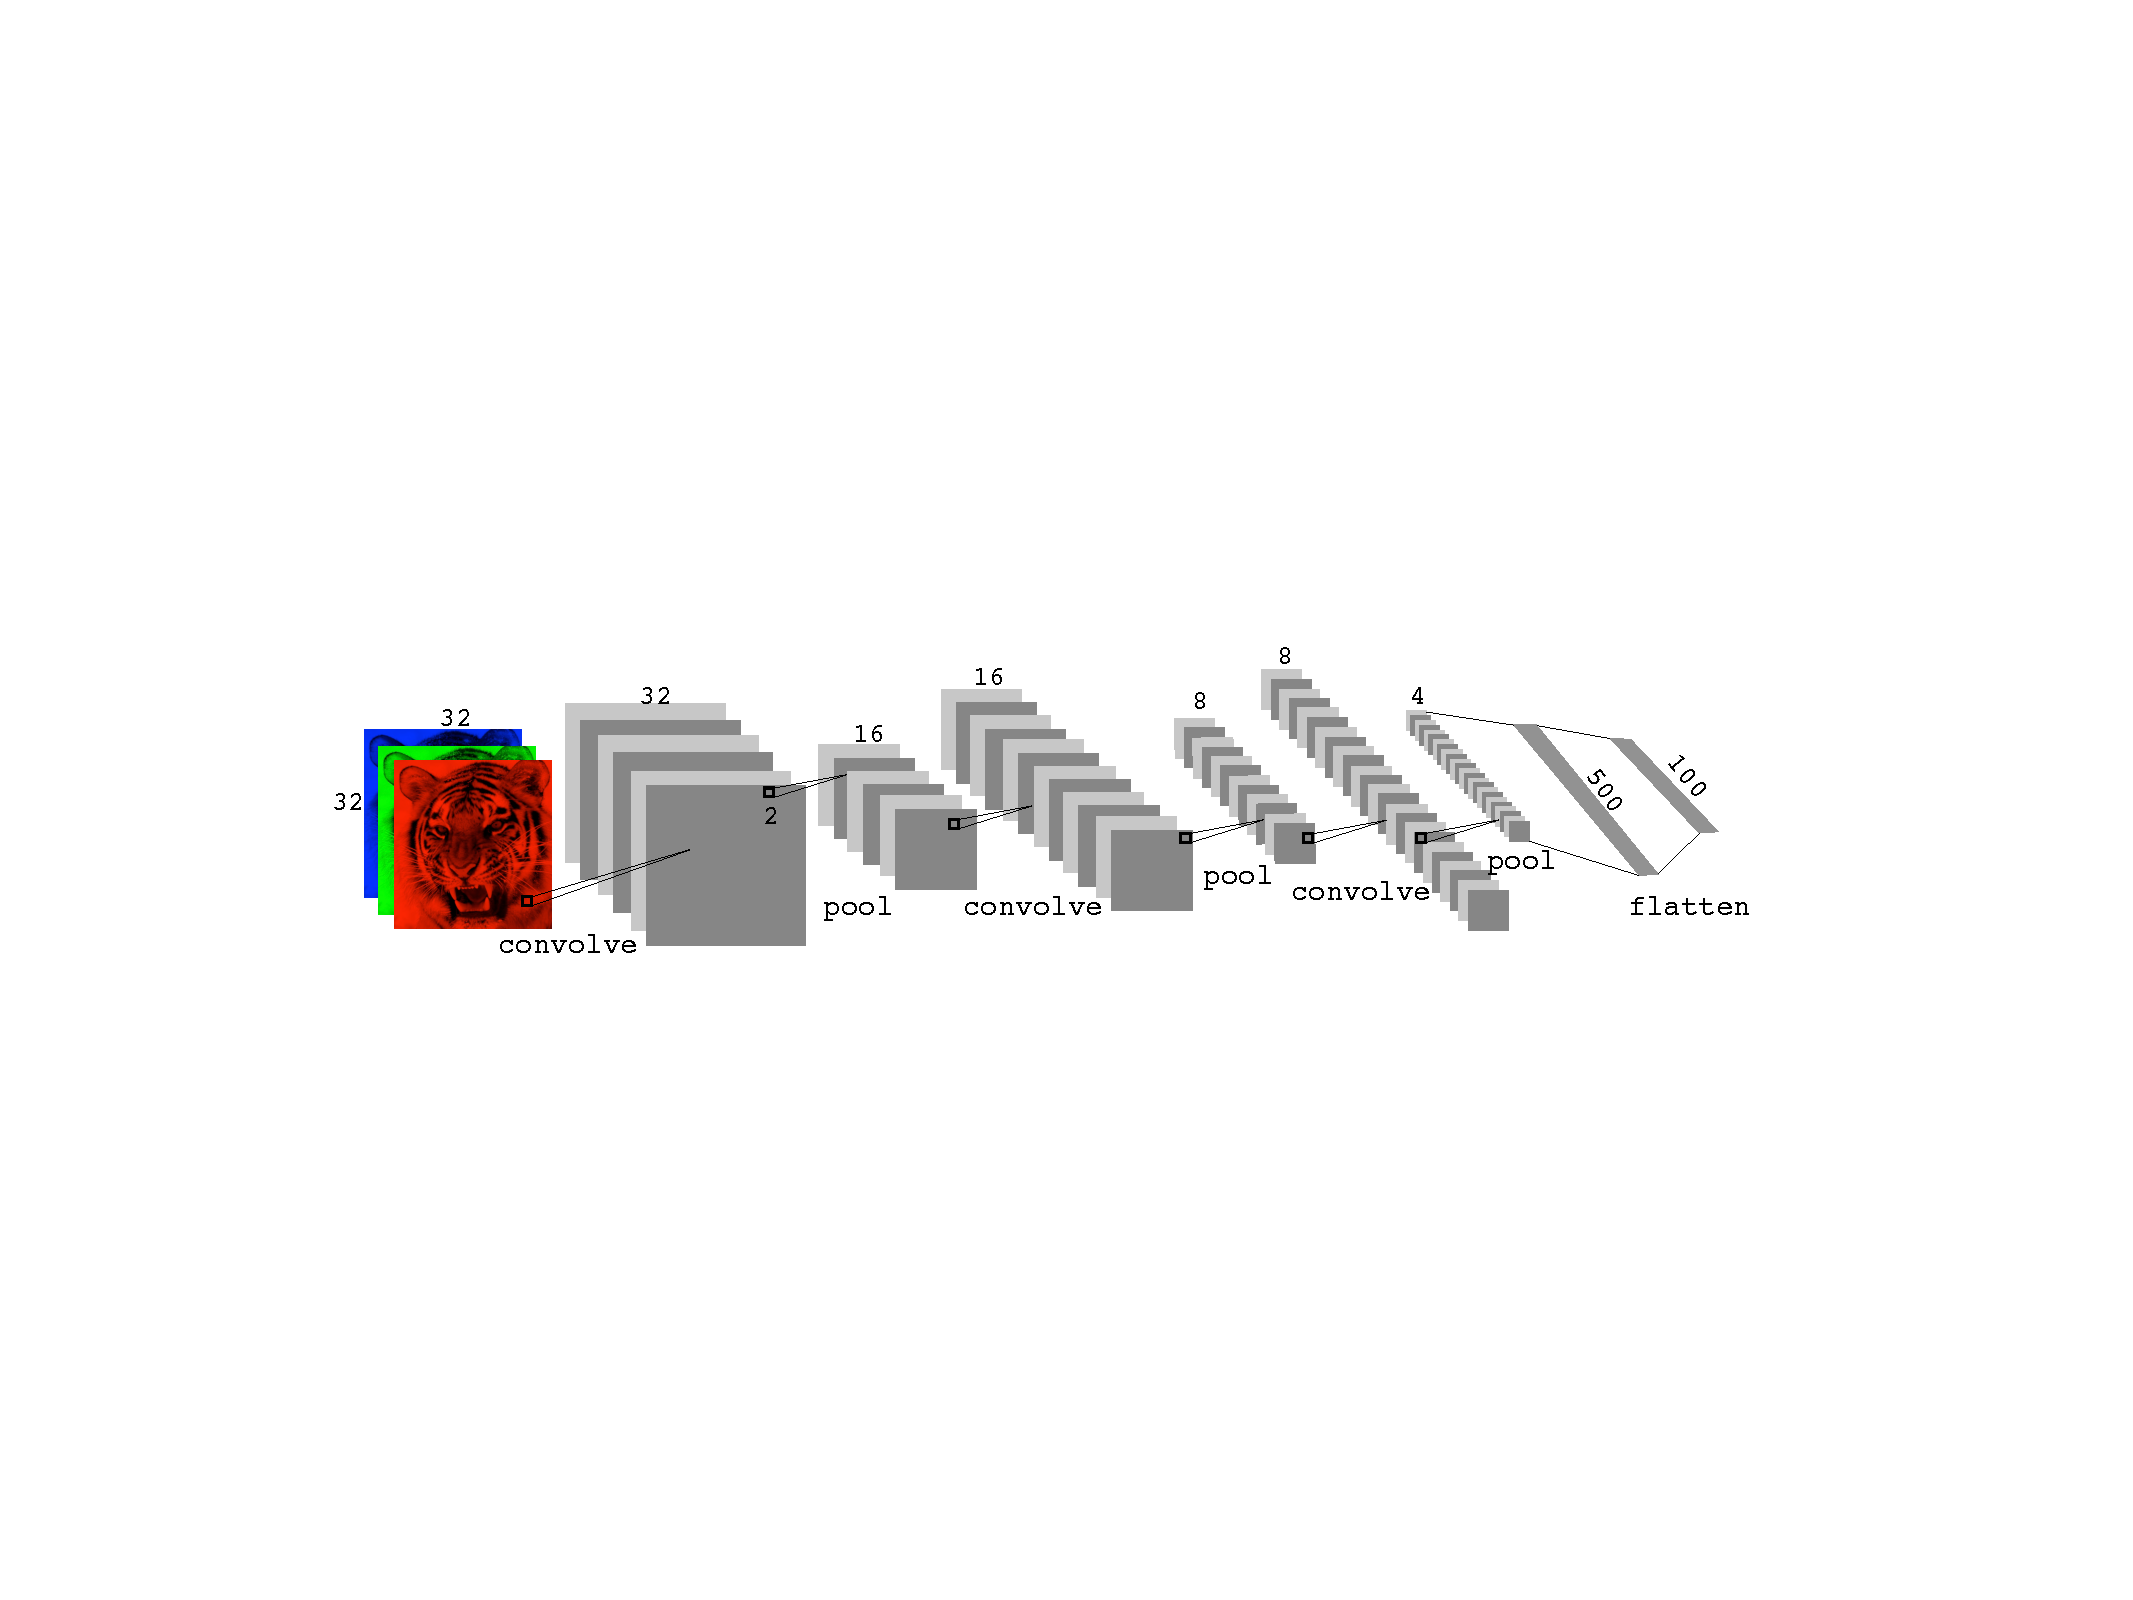
\includegraphics[width=0.92\textwidth,height=0.52\textheight,keepaspectratio]{10_8.pdf}
  \end{center}
  \begin{takeaway}
    The pattern repeats: convolutions extract local features, pooling shrinks the
    maps, and a final dense layer classifies. Early layers learn edges; deeper
    layers assemble them into whole objects.
  \end{takeaway}
  \islpsource{Figure 10.8}
\end{frame}

\begin{frame}{Modern CNN tricks}
  \begin{itemize}
    \item \textbf{Batch normalisation}: re-centre and scale each layer's inputs per
          mini-batch --- stabilises and speeds up training.
    \item \textbf{Dropout}: randomly switch off units so the net cannot rely on any
          single one (detailed in the Fitting section).
    \item \textbf{Data augmentation}: random crops, flips, colour jitter --- free
          extra ``images'' that teach invariance.
    \item \textbf{Skip / residual connections} (ResNet): let gradients bypass layers,
          enabling very deep networks.
    \item \textbf{Transfer learning}: reuse features pretrained on ImageNet, then
          fine-tune on your (smaller) task.
  \end{itemize}
  \begin{takeaway}
    These tricks turned CNNs from finicky to reliable. Most are cheap to add and
    mainly improve \emph{generalisation}.
  \end{takeaway}
\end{frame}


% ------------------------------------------------------------
\begin{frame}{Exercise 10.4 --- CNN layer arithmetic [Math]}
\begin{exercise}
  A colour image of size $32 \times 32 \times 3$ is fed to a
  convolutional layer with $16$ filters, each $5 \times 5$, stride
  $1$, no padding (``valid''). Recall the spatial-size formula
  \[
    O = \left\lfloor\frac{W - F + 2P}{S}\right\rfloor + 1 .
  \]
  \begin{enumerate}
    \item Compute the output volume (height, width, depth) of the
          conv layer.
    \item Compute the number of trainable parameters in the conv layer
          (include biases).
    \item A $2 \times 2$ max-pooling layer (stride $2$) follows. What
          is its output volume and how many parameters does it add?
    \item Redo part (1) if instead padding $P = 2$ (``same'') is used.
  \end{enumerate}
\end{exercise}
\end{frame}

\begin{frame}{Solution --- Exercise 10.4 (1/2)}
\begin{solutionbox}
  \textbf{Part 1 --- conv output.} With $W = 32$, $F = 5$, $P = 0$,
  $S = 1$:
  \[
    O = \frac{32 - 5 + 0}{1} + 1 = 28 .
  \]
  Each filter slides over the image and produces \emph{one} $28 \times 28$
  feature map, so depth $=$ number of filters: the output volume is
  $28 \times 28 \times 16$.

  \medskip
  \textbf{Part 2 --- conv parameters.} Each filter spans the full
  input depth: $5 \times 5 \times 3 = 75$ weights, $+1$ bias $= 76$
  per filter. With $16$ filters:
  \[
    16 \times 76 = \boxed{1216} \text{ parameters.}
  \]
  \emph{Why so few?} A dense layer from the $32 \times 32 \times 3 = 3072$
  inputs to the same $28 \times 28 \times 16 = 12\,544$ outputs would need
  $3072 \times 12\,544 + 12\,544 \approx 38.5$ million parameters --- weight
  sharing cuts that by a factor of about $30\,000$.
\end{solutionbox}
\end{frame}

\begin{frame}{Solution --- Exercise 10.4 (2/2)}
\begin{solutionbox}
  \textbf{Part 3 --- pooling.} Max-pooling with $F = 2$, $S = 2$:
  \[
    O = \frac{28 - 2}{2} + 1 = 14 ,
  \]
  giving $14 \times 14 \times 16$: pooling acts on each of the $16$ channels
  separately, so depth is preserved. It has \textbf{no} trainable
  parameters --- it only takes a maximum.

  \medskip
  \textbf{Part 4 --- with padding $P = 2$.}
  \[
    O = \frac{32 - 5 + 2(2)}{1} + 1 = \frac{31}{1} + 1 = 32 .
  \]
  Output $32 \times 32 \times 16$: ``same'' padding preserves the
  spatial size. In general, stride-$1$ ``same'' padding takes
  $P = (F-1)/2$ --- here $(5-1)/2 = 2$ --- so conv layers can be stacked
  without shrinking the maps.

  \medskip
  \textit{Common mistake: adding a $+2P$ term for the pooling layer (it uses
  $P = 0$) or forgetting to divide by the stride \emph{before} adding $1$.}
\end{solutionbox}
\end{frame}





% ============================================================
\section{Sequences}
% ============================================================

\begin{frame}{Recurrent neural networks (RNNs)}
  Process sequences $x_1, \ldots, x_T$ by carrying a hidden state forward:
  \[
    \boxed{\,h_t = g\!\left(W_x\, x_t + W_h\, h_{t-1} + b\right).\,}
  \]
  \begin{readme}[Reading the recurrence]
    \begin{itemize}
      \item $x_t$: input at step $t$; \ $h_t$: hidden state (``memory'') at step $t$.
      \item $W_x$: weights on the new input; \ $W_h$: weights on the previous state
            $h_{t-1}$; \ $b$: bias.
      \item The \emph{same} $W_x,W_h,b$ are reused at every step --- weight sharing
            across time.
    \end{itemize}
  \end{readme}
  \begin{takeaway}
    Suitable for time series, text, audio. Plain RNNs suffer from
    vanishing/exploding gradients; LSTM and GRU add gating to carry long-range
    information.
  \end{takeaway}
\end{frame}

\begin{frame}{An RNN unrolled in time}
  \begin{center}
    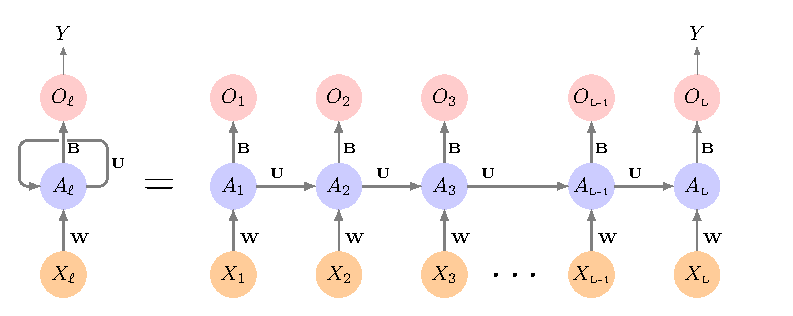
\includegraphics[width=0.85\textwidth,height=0.50\textheight,keepaspectratio]{10_12.pdf}
  \end{center}
  \begin{takeaway}
    Unrolling shows the recurrence as a deep feed-forward net that reuses the same
    weights at every step; training uses backpropagation ``through time''.
  \end{takeaway}
  \islpsource{Figure 10.12}
\end{frame}



% ============================================================
\section{Fitting}
% ============================================================

\begin{frame}{Loss and optimisation}
  Choose a loss $L(\theta) = \sum_i \ell(y_i, \hat y_i; \theta)$ and
  minimise by stochastic gradient descent:
  \[
    \theta \leftarrow \theta - \eta\,\nabla_\theta \ell_{\mathrm{minibatch}}(\theta).
  \]
  \begin{readme}[Reading the update]
    \begin{itemize}
      \item $\theta$: all weights and biases; \ $\nabla_\theta \ell$: gradient
            (steepest-\emph{ascent} direction) of the loss.
      \item Step \emph{against} the gradient, scaled by the learning rate $\eta$
            (too large diverges, too small crawls --- see Exercise 10.5).
      \item ``Stochastic'': each step uses one random mini-batch (32/64/128) --- a
            cheap, noisy estimate of the full-data gradient.
      \item Modern optimisers add memory: SGD${+}$momentum, Adam, RMSprop.
    \end{itemize}
  \end{readme}
\end{frame}

\begin{frame}{Training a network: descent and early stopping}
  \begin{center}
    
\includegraphics[width=0.92\textwidth,height=0.58\textheight,keepaspectratio]{ch10_training.png}
  \end{center}
  \begin{takeaway}
    Gradient descent steps downhill along the loss surface (left). In practice, watch training \emph{and} validation loss and stop at the validation minimum, before overfitting sets in (right).
  \end{takeaway}
\end{frame}

\begin{frame}{Gradient descent on a loss surface: the real path}
  \begin{center}
\includegraphics[width=0.88\textwidth,height=0.52\textheight,keepaspectratio]{ch10_x_gradient_descent.png}\end{center}
  \begin{takeaway}Each step is perpendicular to the local contour: with $\eta=0.05$ the loss falls from $27$ to $0.05$ in $25$ steps --- fast down the steep $w_2$ axis, then a crawl along the flat valley --- while the too-large $\eta=0.115$ overshoots and zigzags in the steep direction.\end{takeaway}
\end{frame}


\begin{frame}{Regularisation in deep learning}
  Modern networks can have more parameters than data points but still
  generalise. Why?
  \begin{readme}
    \begin{itemize}
      \item Implicit regularisation by SGD.
      \item Dropout, weight decay ($\ell_2$), early stopping.
      \item Data augmentation.
      \item Architecture choice is itself a strong inductive bias.
    \end{itemize}
  \end{readme}
\end{frame}

\begin{frame}{Dropout: randomly switch off units during training}
  \begin{center}
  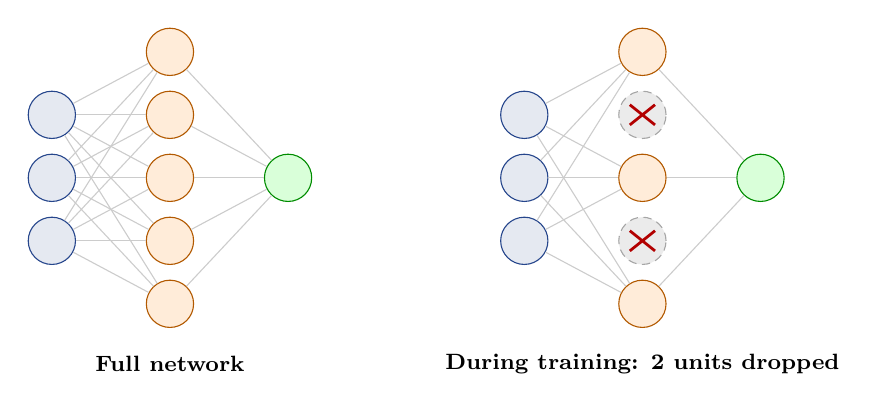
\begin{tikzpicture}[x=1cm,y=0.8cm,>={Stealth[length=1.6mm]},
      unit/.style={circle,draw=accent,fill=accent!12,minimum size=6mm,inner sep=0pt},
      hid/.style={circle,draw=orange!70!black,fill=orange!15,minimum size=6mm,inner sep=0pt},
      outn/.style={circle,draw=green!55!black,fill=green!15,minimum size=6mm,inner sep=0pt},
      off/.style={circle,draw=black!35,fill=black!8,minimum size=6mm,inner sep=0pt,densely dashed},
      e/.style={draw=black!20,line width=0.4pt}]
    % LEFT: full network
    \foreach \i/\y in {1/1,2/0,3/-1} \node[unit] (LI\i) at (0,\y) {};
    \foreach \i/\y in {1/2,2/1,3/0,4/-1,5/-2} \node[hid] (LH\i) at (1.5,\y) {};
    \node[outn] (LO) at (3,0) {};
    \foreach \i in {1,2,3}\foreach \j in {1,2,3,4,5} \draw[e] (LI\i) -- (LH\j);
    \foreach \j in {1,2,3,4,5} \draw[e] (LH\j) -- (LO);
    \node[font=\footnotesize\bfseries] at (1.5,-2.95) {Full network};
    % RIGHT: with dropout
    \begin{scope}[shift={(6,0)}]
      \foreach \i/\y in {1/1,2/0,3/-1} \node[unit] (RI\i) at (0,\y) {};
      \foreach \i/\y in {1/2,3/0,5/-2} \node[hid] (RH\i) at (1.5,\y) {};
      \foreach \i/\y in {2/1,4/-1} \node[off] (RH\i) at (1.5,\y) {};
      \node[outn] (RO) at (3,0) {};
      \foreach \i in {1,2,3}\foreach \j in {1,3,5} \draw[e] (RI\i) -- (RH\j);
      \foreach \j in {1,3,5} \draw[e] (RH\j) -- (RO);
      \foreach \y in {1,-1} \draw[red!70!black,line width=1pt]
         (1.5-0.16,\y+0.16)--(1.5+0.16,\y-0.16) (1.5-0.16,\y-0.16)--(1.5+0.16,\y+0.16);
      \node[font=\footnotesize\bfseries] at (1.5,-2.95) {During training: 2 units dropped};
    \end{scope}
  \end{tikzpicture}
  \end{center}
  \begin{takeaway}
    On each mini-batch, every hidden unit is kept with probability $1-\rho$ and otherwise
    \emph{zeroed}, so the net cannot lean on any single unit and learns redundant,
    robust features. At test time all units are used (weights rescaled).
  \end{takeaway}
\end{frame}



% ------------------------------------------------------------
\begin{frame}{Exercise 10.5 --- One gradient-descent step [Math]}
\begin{exercise}
  Consider minimising the loss $L(w) = (w - 3)^2$ by gradient
  descent, $w \leftarrow w - \eta\, L'(w)$, starting from $w = 2$.
  \begin{enumerate}
    \item Write $L'(w)$ and evaluate it at $w = 2$.
    \item Perform one update with learning rate $\eta = 0.1$.
    \item Show that the update rule for the \emph{error} $e = w - 3$
          is $e \leftarrow (1 - 2\eta)\,e$, and deduce the range of
          $\eta$ for which gradient descent converges.
    \item What happens with $\eta = 1.5$? Interpret.
  \end{enumerate}
\end{exercise}
\end{frame}

\begin{frame}{Solution --- Exercise 10.5 (1/2)}
\begin{solutionbox}
  \textbf{Part 1 --- gradient.}
  $L'(w) = 2(w - 3)$, so $L'(2) = 2(2 - 3) = -2$.

  \medskip
  \textbf{Part 2 --- one step ($\eta = 0.1$).}
  \[
    w \leftarrow 2 - 0.1 \times (-2) = 2 + 0.2 = 2.2 .
  \]
  We moved from $2$ toward the minimiser $w^\star = 3$: good.

  \medskip
  \textbf{Part 3 --- convergence range.} Substituting $L'(w) = 2(w-3)$
  into the update,
  \[
    w \leftarrow w - \eta\, 2(w - 3)
    \;\Longrightarrow\;
    (w - 3) \leftarrow (w - 3) - 2\eta (w - 3) = (1 - 2\eta)(w - 3).
  \]
  So $e_{t+1} = (1 - 2\eta)\, e_t$, hence $e_t = (1 - 2\eta)^t\, e_0$: a
  geometric sequence, which dies out iff its ratio satisfies
  $|1 - 2\eta| < 1$, i.e.
  \[
    0 < \eta < 1 .
  \]
  With $\eta = 0.1$ the ratio is $0.8$ --- each step removes $20\%$ of the
  remaining error.
\end{solutionbox}
\end{frame}

\begin{frame}{Solution --- Exercise 10.5 (2/2)}
\begin{solutionbox}
  \textbf{Part 4 --- $\eta = 1.5$.} Then $1 - 2\eta = -2$, so
  $|1 - 2\eta| = 2 > 1$: the error \emph{doubles} each step and flips
  sign. Concretely $w \leftarrow 2 - 1.5(-2) = 5$; now
  $|5 - 3| = 2 > |2 - 3| = 1$, and iterating,
  \[
    \begin{array}{c|cccc}
      t & 0 & 1 & 2 & 3 \\ \hline
      w_t & 2 & 5 & -1 & 11 \\
      e_t = w_t - 3 & -1 & 2 & -4 & 8
    \end{array}
  \]
  The steps overshoot the minimum ever more wildly: gradient
  descent \textbf{diverges}. This is the classic ``learning rate too
  large'' failure --- $\eta$ trades off speed against stability.

  \medskip
  \textbf{Interpretation.} The extremes are instructive: $\eta = 0.5$ makes
  the ratio $1 - 2\eta = 0$ and lands on $w^\star = 3$ in \emph{one} step
  (possible only because this loss is exactly quadratic), while a tiny
  $\eta$ converges but crawls.

  \medskip
  \textit{Common mistake: concluding ``smaller is always safer, so smaller
  is better'' --- at $\eta = 0.01$ the ratio is $0.98$ and hundreds of steps
  are needed here.}
\end{solutionbox}
\end{frame}

% ============================================================
\section{Python Lab}

\begin{frame}{Python lab --- run it live in the notebook}
  \begin{labnote}[Companion notebook: \texttt{chapter\_10\_lab.ipynb}]
    The code in this section is meant to be \textbf{demonstrated live}. Open the companion Jupyter notebook and run it cell by cell:
    \begin{itemize}
      \item building a small multilayer perceptron in \textbf{PyTorch};
      \item the data pipeline, model definition, and training loop;
      \item evaluating and tuning the network.
    \end{itemize}
    Requires \texttt{torch}; the notebook ends with hands-on exercises.
  \end{labnote}
\end{frame}


% ============================================================

\begin{frame}[fragile]{An MLP in PyTorch}
  \begin{lstlisting}
import torch
from torch import nn, optim

class MLP(nn.Module):              # a model = a subclass of nn.Module
    def __init__(self, p, k=64, K=2):   # p inputs, k hidden units, K classes
        super().__init__()
        self.net = nn.Sequential(       # layers applied in order:
            nn.Linear(p, k),            #   affine map  W x + b   (p -> k)
            nn.ReLU(),                  #   nonlinearity  max(0, z)
            nn.Dropout(0.2),            #   randomly zero 20% of units (regularises)
            nn.Linear(k, k), nn.ReLU(), nn.Dropout(0.2),   # second hidden layer
            nn.Linear(k, K))            #   output layer: K logits (no softmax here)
    def forward(self, x):               # forward pass: how inputs become outputs
        return self.net(x)

model = MLP(p=Xtr.shape[1])             # build the network for our p predictors
opt = optim.Adam(model.parameters(), lr=1e-3)   # optimiser: Adam, learning rate 0.001
  \end{lstlisting}
\end{frame}


% ------------------------------------------------------------
\begin{frame}[fragile]{Exercise 10.6 --- Softmax and cross-entropy [Python]}
\begin{exercise}
  A 3-class classifier outputs the logits
  $z = (2.0,\; 1.0,\; 0.1)$ for one observation whose true label is
  class $0$.
  \begin{enumerate}
    \item By hand, compute the softmax probabilities
          $p_k = e^{z_k} / \sum_j e^{z_j}$.
    \item Compute the cross-entropy loss
          $\ell = -\log p_{y}$ for the true class $y = 0$.
    \item Write short NumPy code that reproduces both and prints them.
  \end{enumerate}
\end{exercise}
\end{frame}

\begin{frame}{Solution --- Exercise 10.6 (1/3)}
\begin{solutionbox}
  \textbf{Method.} Softmax exponentiates each logit (making it positive) and
  divides by the sum, turning arbitrary scores into a probability vector;
  cross-entropy then scores only the probability given to the \emph{true} class.

  \smallskip
  \textbf{Step 1 --- exponentiate.}
  \[
    e^{2.0} = 7.389,\quad e^{1.0} = 2.718,\quad e^{0.1} = 1.105,
    \qquad \textstyle\sum = 11.212 .
  \]
  \textbf{Step 2 --- softmax probabilities.}
  \[
    p = \left(\tfrac{7.389}{11.212},\; \tfrac{2.718}{11.212},\;
              \tfrac{1.105}{11.212}\right)
      = (0.659,\; 0.242,\; 0.099).
  \]
  \emph{Check:} the three probabilities sum to $1.000$.

  \smallskip
  \textbf{Step 3 --- cross-entropy for $y = 0$.}
  \[
    \ell = -\log p_0 = -\log(0.659) = 0.417 .
  \]
  \textit{Common mistake: using $\log_{10}$ instead of the natural log ($-\ln 0.659 = 0.417$).}
\end{solutionbox}
\end{frame}

\begin{frame}[fragile]{Solution --- Exercise 10.6 (2/3)}
\begin{solutionbox}
\begin{lstlisting}
import numpy as np                # numerics library

z = np.array([2.0, 1.0, 0.1])     # logits from the network
p = np.exp(z) / np.exp(z).sum()   # softmax: exponentiate, normalise
print("probs:", np.round(p, 3))   # [0.659 0.242 0.099]

y = 0                             # true class label
loss = -np.log(p[y])              # cross-entropy = -log(true-class prob)
print("loss:", round(float(loss), 3))   # 0.417
\end{lstlisting}
\end{solutionbox}
\end{frame}

\begin{frame}{Solution --- Exercise 10.6 (3/3)}
\begin{solutionbox}[Interpretation]
  The model assigns the highest probability ($0.659$) to the correct
  class, so the loss is modest. A perfect prediction ($p_0 = 1$)
  gives loss $0$; a confidently wrong prediction sends
  $-\log p_0 \to \infty$ --- cross-entropy punishes confident errors
  hardest, exactly the gradient signal a classifier needs.

  \medskip
  \textbf{Why the ``log-sum-exp'' trick works.} Softmax is shift-invariant:
  dividing top and bottom by $e^{c}$ gives $p_k = e^{z_k - c}/\sum_j e^{z_j - c}$,
  unchanged for any $c$. Choosing $c = \max_k z_k = 2.0$ here,
  \[
    e^{0} = 1,\quad e^{-1} = 0.368,\quad e^{-1.9} = 0.150,\qquad
    p = \tfrac{1}{1.518}\,(1,\; 0.368,\; 0.150) = (0.659,\; 0.242,\; 0.099),
  \]
  the same probabilities --- but every exponent is now $\le 0$, so nothing
  can overflow no matter how large the logits get.

  \medskip
  \textit{Common mistake: applying softmax yourself and then calling PyTorch's
  \texttt{nn.CrossEntropyLoss} --- that loss already includes the softmax and
  expects raw logits; softmaxing twice silently distorts the loss.}
\end{solutionbox}
\end{frame}

% ------------------------------------------------------------
% EXTENDED (INTEGRATIVE) EXERCISE 10.3 --- MLP overfitting + regularisation
\begin{frame}{Extended Exercise 10.3 --- Overfitting and regularisation [Python]}
\begin{longexercise}
  Fit a \textbf{PyTorch} multilayer perceptron to the \texttt{Default} data,
  \emph{watch it overfit}, then tame it. Encode \texttt{student} as $0/1$, standardise
  \texttt{(balance, income, student)}, and predict \texttt{default}.
  \begin{enumerate}
    \item Train on a \emph{small} subset ($n_{\text{train}}=200$) with a wide MLP
          (two hidden layers of $128$, no dropout) and no weight decay, recording the
          training and validation cross-entropy after every epoch.
    \item Where does the validation loss turn upward, and what does the training loss do?
    \item Refit with strong L2 regularisation
          (\texttt{weight\_decay=0.1} in Adam); compare the validation
          loss and say what \emph{early stopping} would choose.
  \end{enumerate}
\end{longexercise}
\end{frame}

\begin{frame}[fragile]{Solution --- Extended Exercise 10.3 (1/3)}
\begin{solutionbox}[Code: load / standardise / convert to tensors]
\begin{lstlisting}[basicstyle=\ttfamily\scriptsize]
import pandas as pd, torch
from torch import nn, optim
from sklearn.preprocessing import StandardScaler
from sklearn.model_selection import train_test_split

df = pd.read_csv("Default.csv")
df["y"]       = (df["default"] == "Yes").astype(int)  # response -> 0/1
df["student"] = (df["student"] == "Yes").astype(int)  # dummy-code student
X = df[["balance", "income", "student"]].astype(float).values
Xtr, Xte, ytr, yte = train_test_split(X, df["y"].values,
    train_size=200, random_state=0, stratify=df["y"])  # tiny train set!
sc = StandardScaler().fit(Xtr)          # scale using TRAIN stats only
Xtr, Xte = sc.transform(Xtr), sc.transform(Xte)
# PyTorch works on tensors: features float32, labels int64
Xtr, Xte = map(lambda a: torch.tensor(a, dtype=torch.float32), (Xtr, Xte))
ytr, yte = map(lambda a: torch.tensor(a, dtype=torch.int64), (ytr, yte))
\end{lstlisting}
\end{solutionbox}
\end{frame}

\begin{frame}[fragile]{Solution --- Extended Exercise 10.3 (2/3)}
\begin{solutionbox}[Code: train and record the loss after every epoch]
\begin{lstlisting}[basicstyle=\ttfamily\scriptsize\linespread{0.88}\selectfont]
def curve(weight_decay, epochs=400):
    torch.manual_seed(1)                       # reproducible weights
    net = nn.Sequential(nn.Linear(3,128), nn.ReLU(),    # wide MLP
        nn.Linear(128,128), nn.ReLU(), nn.Linear(128,2))
    loss_fn = nn.CrossEntropyLoss()            # softmax + log-loss in one
    opt = optim.Adam(net.parameters(), lr=1e-2,
                     weight_decay=weight_decay)  # L2 penalty lives here
    tr, va = [], []
    for _ in range(epochs):              # 1 epoch = 1 full-batch step here
        opt.zero_grad()                          # reset gradients
        loss = loss_fn(net(Xtr), ytr)            # forward pass on TRAIN
        loss.backward(); opt.step()              # backprop + update
        with torch.no_grad():                    # eval: no gradients
            tr.append(loss.item()); va.append(loss_fn(net(Xte), yte).item())
    return tr, va
tr0, va0 = curve(0.0)    # unregularised -> memorises the 200 points
tr1, va1 = curve(0.1)    # strong weight decay (L2)
\end{lstlisting}
\end{solutionbox}
\end{frame}

\begin{frame}{Solution --- Extended Exercise 10.3 (3/3)}
\begin{solutionbox}[Typical result and interpretation]
  \textbf{Typical values} (exact numbers vary with seed and version):
  \begin{center}\ttfamily\footnotesize
  unreg:\ train $\to$ 0.00\quad val-min $\approx$ 0.10 (early epochs)\quad val-final $\approx$ 0.4--0.5\\[2pt]
  decay:\ train $\approx$ 0.10\quad val \emph{lower and flat} $\approx$ 0.09
  \end{center}
  \begin{itemize}
    \item \emph{Unregularised:} training loss dives toward $0$ (the net \textbf{memorises}
          the $200$ points), but validation loss bottoms out within the first few dozen
          epochs and then \textbf{climbs} several-fold --- textbook overfitting.
    \item \emph{Weight decay:} training loss stays higher, yet validation loss is
          \emph{lower and flat}: the L2 penalty trades a little fit for much
          better generalisation.
    \item \emph{Early stopping} halts at the validation minimum --- a free regulariser
          needing no extra penalty term.
  \end{itemize}
  \textit{Same recipe as the companion notebook} (\texttt{chapter\_10\_lab.ipynb});
  there the MLP adds dropout and mini-batches via \texttt{DataLoader}.
\end{solutionbox}
\end{frame}

% ============================================================
\section{Summary}
% ============================================================

\begin{frame}{Chapter 10 in one slide}
  \begin{block}{What we accomplished}
    Surveyed the modern deep-learning landscape and connected it to
    the classical methods of the earlier chapters.
  \end{block}
  \begin{itemize}
    \item Single- and multilayer perceptrons.
    \item Convolutional networks for images.
    \item Recurrent networks and transformers.
    \item Optimisation: SGD, momentum, Adam, backpropagation.
    \item Regularisation: dropout, weight decay, early stopping.
  \end{itemize}
\end{frame}

\begin{frame}{Key formulas at a glance}
  \footnotesize
  \begin{description}
    \item[Neuron] $a=g\!\big(\textstyle\sum_j w_j x_j+b\big)$, activation $g$.
    \item[Single hidden layer] $f(x)=\beta_0+\sum_{k=1}^{K}\beta_k\,g\!\big(w_{k0}+\sum_j w_{kj}x_j\big)$.
    \item[Activations] ReLU $g(z)=\max(0,z)$; \ sigmoid $\sigma(z)=\dfrac{1}{1+e^{-z}}$; \ softmax $\dfrac{e^{z_m}}{\sum_\ell e^{z_\ell}}$.
    \item[Loss] regression $\sum_i(y_i-f(x_i))^2$; \ classification $-\sum_i\sum_k y_{ik}\log f_k(x_i)$.
    \item[Gradient descent] $\theta \leftarrow \theta-\eta\,\nabla_\theta L(\theta)$ \ (learning rate $\eta$).
    \item[Conv output] size $=\big\lfloor (W-F+2P)/S\big\rfloor+1$ \ (input $W$, filter $F$, pad $P$, stride $S$).
  \end{description}
\end{frame}

\begin{frame}{Vocabulary checklist}
  \footnotesize
  \begin{tabular}{ll}
    \toprule
    \textbf{Term} & \textbf{Meaning} \\
    \midrule
    Activation function & Element-wise nonlinearity (ReLU, tanh, sigmoid) \\
    Hidden unit & One node in a hidden layer \\
    Backpropagation & Reverse-mode automatic differentiation \\
    SGD / momentum & Stochastic gradient + velocity term \\
    Adam & Adaptive per-parameter learning rates \\
    Dropout & Random unit muting during training \\
    Weight decay & $\ell_2$ penalty on weights \\
    CNN & Conv + pool + dense layers for images \\
    RNN / LSTM & Sequential models with hidden state \\
    Transformer & Self-attention based sequence model \\
    Double descent & Test-error second dip \\
    \bottomrule
  \end{tabular}
\end{frame}

\begin{frame}{Decision rules of thumb}
  \begin{itemize}
    \item Tabular data ($n < 10^5$, $p < 10^3$): try gradient
          boosting first.
    \item Images: pretrained CNN (ResNet, EfficientNet) and
          fine-tune.
    \item Text: pretrained transformer; fine-tune only the head when
          $n$ is small.
    \item Always normalise inputs and labels.
    \item Track training and validation loss together.
    \item Save the best-validation checkpoint.
  \end{itemize}
\end{frame}

\begin{frame}{Common pitfalls}
  \begin{alertblock}{Don't}
    \begin{enumerate}
      \item Compare a deep network to a poorly tuned baseline.
      \item Forget to shuffle training data before each epoch.
      \item Use too high a learning rate (loss explodes).
      \item Trust accuracy without checking calibration.
      \item Skip data augmentation for image / audio tasks.
      \item Re-use the validation set for many tuning rounds.
    \end{enumerate}
  \end{alertblock}
\end{frame}

\begin{frame}{What's next}
  Chapter 13: \emph{Multiple Testing}.
  \begin{itemize}
    \item The multiple-comparisons problem and the family-wise error rate.
    \item Bonferroni and Holm corrections.
    \item The false discovery rate and Benjamini-Hochberg.
  \end{itemize}
\end{frame}


% ============================================================
\appendix
\AtBeginSection[]{}
\section{Appendix: optional and advanced material}
% ============================================================

\begin{frame}{Appendix --- what is in here, and why}
  \small
  Nothing in the appendix is needed to follow the chapter: each slide is a
  formal derivation, a longer worked exercise, or a side topic. Read it when
  you want the full story, or when a later chapter sends you back here.
  \begin{block}{Contents of the appendix}
    \begin{itemize}
      \item \textbf{CNN architecture arithmetic (Extended Exercise 10.2)} --- shapes and parameter counts through a whole network. Exercise 10.4 does the same arithmetic for a single layer.
      \item \textbf{Transformers} --- self-attention in one slide. Outside the scope of ISLP Chapter 10; here so that the word is not a mystery.
      \item \textbf{Backpropagation} --- the chain rule that computes the gradients. Every framework does this for you; the main deck keeps what you must know --- that training is gradient descent on a loss.
      \item \textbf{Double descent} --- why very over-parameterised models can improve again past the interpolation point. A genuinely advanced topic.
    \end{itemize}
  \end{block}
\end{frame}

% ------------------------------------------------------------
% EXTENDED (INTEGRATIVE) EXERCISE 10.2 --- CNN dimension + parameter arithmetic
\begin{frame}{Extended Exercise 10.2 --- CNN architecture arithmetic [Math]}
\begin{longexercise}
  A $64\times64\times3$ RGB image passes through the stack below (convolutions use the
  padding shown; pooling is max-pooling, no padding). Recall
  $O=\big\lfloor(W-F+2P)/S\big\rfloor+1$.
  \begin{center}\footnotesize
  \begin{tabular}{lccc}
    \toprule
    Layer & Kernel & Stride / Pad & Filters \\
    \midrule
    Conv1 & $3\times3$ & $1\,/\,1$ & $32$ \\
    Pool1 & $2\times2$ & $2\,/\,0$ & --- \\
    Conv2 & $3\times3$ & $1\,/\,1$ & $64$ \\
    Pool2 & $2\times2$ & $2\,/\,0$ & --- \\
    Dense & softmax & --- & $10$ \\
    \bottomrule
  \end{tabular}
  \end{center}
  \begin{enumerate}
    \item Give the output volume ($H\times W\times$ depth) after each layer.
    \item Count the learnable parameters of every layer, and the total.
    \item What input region does one unit of the last conv map see (receptive field)?
  \end{enumerate}
\end{longexercise}
\end{frame}

\begin{frame}{Solution --- Extended Exercise 10.2 (1/3)}
\begin{solutionbox}[Spatial dimensions]
  Apply $O=(W-F+2P)/S+1$ to $H$ and $W$; depth $=$ number of filters (pooling keeps
  depth).
  \[
    \begin{aligned}
      \text{Conv1}:&\ (64-3+2)/1+1=64 &&\Rightarrow\ 64\times64\times32,\\
      \text{Pool1}:&\ (64-2)/2+1=32   &&\Rightarrow\ 32\times32\times32,\\
      \text{Conv2}:&\ (32-3+2)/1+1=32 &&\Rightarrow\ 32\times32\times64,\\
      \text{Pool2}:&\ (32-2)/2+1=16   &&\Rightarrow\ 16\times16\times64.
    \end{aligned}
  \]
  Flattening the last volume gives $16\times16\times64=16384$ features into the dense
  layer. ``Same'' padding preserves $H,W$; each pool halves them.

  \medskip
  \textit{Common mistake: flattening only $16\times16=256$ features --- the
  depth counts too: $16\times16\times64=16\,384$.}
\end{solutionbox}
\end{frame}

\begin{frame}{Solution --- Extended Exercise 10.2 (2/3)}
\begin{solutionbox}[Learnable parameters]
  A conv filter spans the \emph{full input depth}, so
  $\#=(F^2 d_{\text{in}}+1)\times(\text{\#filters})$; pooling has none.
  \[
    \begin{aligned}
      \text{Conv1}:&\ (3^2\cdot3+1)\times32=28\times32=\mathbf{896},\\
      \text{Conv2}:&\ (3^2\cdot32+1)\times64=289\times64=\mathbf{18\,496},\\
      \text{Dense}:&\ 16384\times10+10=\mathbf{163\,850},\\
      \text{Pool1, Pool2}:&\ 0 .
    \end{aligned}
  \]
  \[
    \text{Total}=896+18\,496+163\,850=\boxed{183\,242}\ \text{parameters.}
  \]
\end{solutionbox}
\end{frame}

\begin{frame}{Solution --- Extended Exercise 10.2 (3/3)}
\begin{solutionbox}[Receptive field and interpretation]
  \textbf{Method.} Track the receptive field $r$ and the jump $j$ (input
  pixels between neighbouring units): a layer with filter $F$ and stride $S$
  updates $r \leftarrow r + (F-1)\,j$, then $j \leftarrow j\,S$. Start at
  $r=1$, $j=1$:
  \[
    \begin{aligned}
      \text{Conv1 } (F{=}3,\ S{=}1):&\ \ r = 1 + 2\times1 = 3, & j &= 1,\\
      \text{Pool1 } (F{=}2,\ S{=}2):&\ \ r = 3 + 1\times1 = 4, & j &= 2,\\
      \text{Conv2 } (F{=}3,\ S{=}1):&\ \ r = 4 + 2\times2 = 8, & j &= 2,\\
      \text{Pool2 } (F{=}2,\ S{=}2):&\ \ r = 8 + 1\times2 = 10, & j &= 4.
    \end{aligned}
  \]
  One unit of the final map therefore sees a $10\times10$ patch of the original image.
  \medskip
  \textbf{Take-aways.} (i) Convolutions are parameter-thrifty: the two conv layers use
  $<20$k weights through \emph{weight sharing}, while the single dense layer holds $164$k
  --- about $89\%$ of the model. (ii) Depth plus pooling grow the receptive field, letting
  deep units assemble local edges into global shapes.
\end{solutionbox}
\end{frame}

\begin{frame}{Transformers (briefly)}
  \begin{takeaway}
    ``Attention is all you need'' (Vaswani et al., 2017). Self-attention
    computes weighted combinations of all positions in a sequence.
    Beats RNNs on most NLP tasks; foundation of modern LLMs.
  \end{takeaway}
  \begin{readme}[Self-attention in one line]
    Each position forms a \emph{query} and compares it against every position's
    \emph{key}; the resulting weights average the \emph{values}. So every output
    token can look directly at every input token --- no matter how far apart, and
    all positions are processed in parallel (unlike an RNN's step-by-step loop).
  \end{readme}
\end{frame}

\begin{frame}{Backpropagation in one slide}
  \begin{readme}[The idea in two passes]
    \begin{itemize}
      \item \textbf{Forward pass}: push $x$ through the layers, caching each
            activation.
      \item \textbf{Backward pass}: send an ``error signal'' $\delta$ from the loss
            back to every weight, multiplying local derivatives (the chain rule).
      \item Each weight's gradient $=$ (error signal at its output) $\times$ (its
            input); shared factors are reused, so the cost is $\approx$ one forward
            pass.
    \end{itemize}
  \end{readme}
  \begin{takeaway}
    Backprop is just the chain rule applied from output back to input --- reverse-mode
    automatic differentiation. Implemented in PyTorch, JAX, TensorFlow, so you rarely
    write it by hand.
  \end{takeaway}
\end{frame}

\begin{frame}{Double descent}
  \begin{center}
    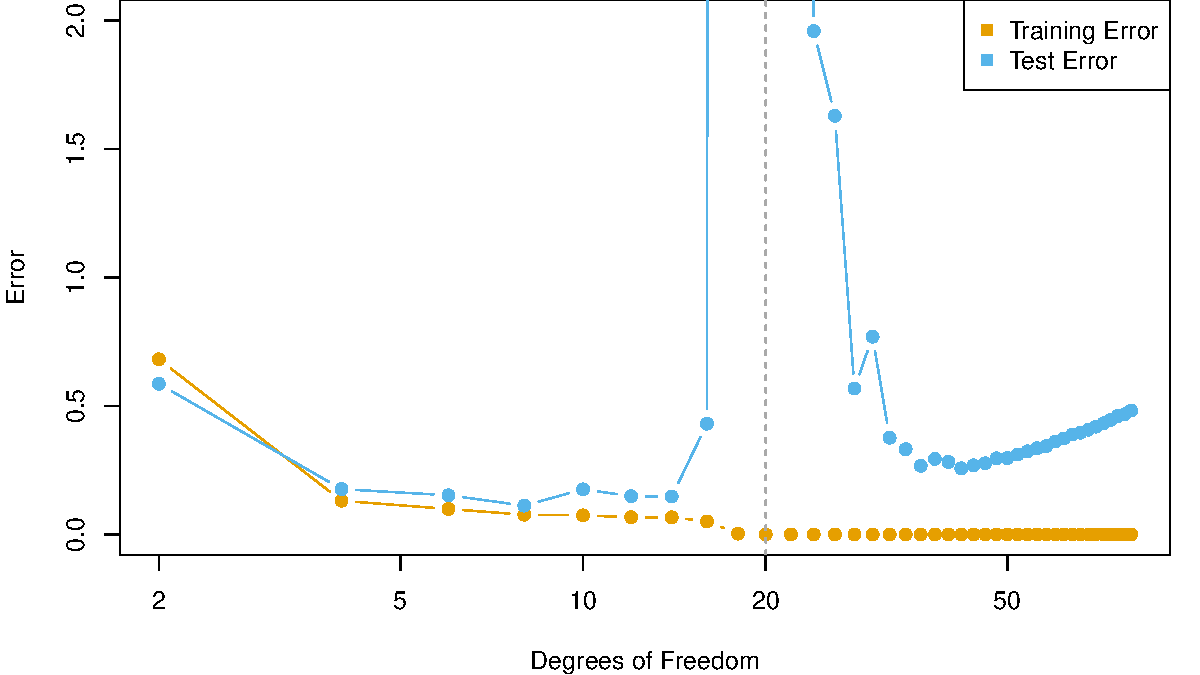
\includegraphics[width=0.85\textwidth,height=0.46\textheight,keepaspectratio]{10_20.pdf}
  \end{center}
  \begin{readme}[Why the second dip]
    Test error first traces the classical U-shape, then peaks at the
    \emph{interpolation threshold} (the model \emph{just} fits the data and is
    unstable), and falls again as extra parameters let SGD pick a smoother
    interpolant.
  \end{readme}
  \islpsource{Figure 10.20}
\end{frame}

\end{document}
